\documentclass[master=cws,masteroption=ai,fleqn,english]{kulemt}
%
% Indien je UTF-8 karakters gebruikt, verwijder "% " uit de volgende lijn
\setup{inputenc=utf8,
% Vul de titel van jouw masterproef hieronder in tussen { en }.
title={Distributed Adversarial Attacks},
%
% Vul hieronder namen in, steeds Voornaam Naam.
% Indien meerdere auteurs, assessoren, assistenten, scheidt hun namen met "\and ".
author={Sander Prenen},
promotor={Prof. dr. ir. W. Joosen \and Dr. ir. D. Preuveneers},
assessor={Ir.\,W. Eetveel\and W. Eetrest},
assistant={V. Rimmer \and I. Tsingenopoulos}
}


% Kies de fonts voor de gewone tekst, bv. Latin Modern
\setup{font=lm}

% Hier kun je dan nog andere pakketten laden of eigen definities voorzien
\usepackage{amsmath, amssymb}
\setlength{\mathindent}{1cm}
\setlength{\parindent}{0mm}
\usepackage{tikz}
\usetikzlibrary{positioning}

\usepackage{pgfplots}
\pgfplotsset{compat=1.16}
\usepackage[caption=false]{subfig}
\usepackage{booktabs}
\usepackage{siunitx}
\usepgfplotslibrary{fillbetween}
\usepgfplotslibrary{external} 
\tikzexternalize[shell escape=-enable-write18]

\usepackage[acronym]{glossaries}
\makenoidxglossaries
\newacronym{ai}{AI}{Artificial Intelligence}
\newacronym{ba}{BA}{Boundary Attack}
\newacronym{bba}{BBA}{Biased Boundary Attack}
\newacronym{relu}{ReLU}{Rectified Linear Unit}
\newacronym{ann}{ANN}{Artificial Neural Network}
\newacronym{cnn}{CNN}{Convolutional Neural Network}
\newacronym{rnn}{RNN}{Recurrent Neural Network}
\newacronym{dnn}{DNN}{Deep Neural Network}
\newacronym{svm}{SVM}{Support Vector Machine}
\newacronym{api}{API}{Application Programming Interface}
\newacronym{fgsm}{FGSM}{Fast Gradient Sign Method}
\newacronym{pso}{PSO}{Particle Swarm Optimization}
\newacronym{ea}{EA}{Evolutionary Algorithm}
\newacronym{dknn}{DkNN}{Deep k-Nearest Neighbors}
\newacronym{ddos}{DDoS}{Distributed Denial of Service}
\newacronym{hsja}{HSJA}{HopSkipJumpAttack}
\newacronym{lstm}{LSTM}{Long Short-Term Memory}
\newacronym{rr}{RR}{Round-Robin}
\newacronym{mrr}{MRR}{Modified Round-Robin}

% Tenslotte wordt hyperref gebruikt voor pdf bestanden.
% Dit mag verwijderd worden voor de af te drukken versie.
\usepackage[pdfusetitle,colorlinks,plainpages=false]{hyperref}

%
%%%%%%%%% Wijzig niets onder deze regel %%%%%%%%

\begin{document}

\begin{preface}

\end{preface}
\begin{abstract}
% Adversarial examples
% Defense
% New attack
% More evasive
%Adversarial attacks craft small perturbations that can be added to inputs, so that they are classified incorrectly by a classifier. Current defensive schemes try to flag these attacks based on the similarity between successive submitted queries. This work aims to implement a new adversarial attack that is able to bypass this detection mechanism. This attack is called PSO-BBA after the two constituent algorithms Particle Swarm Optimization and Biased Boundary Attack \cite{brunner_guessing_2019}. Other improvements, such as distributing the query submission over multiple nodes or grouping attacks together have been explored as well. The final attack is more evasive than current state-of-the-art attacks, but is slightly less efficient. The attacker has to make a trade-off depending on the primary goal of the attack.
Image classification models are prone to adversarial examples. Adversarial examples are perceptually identical to original inputs, but they are classified differently. The examples are crafted using adversarial attack algorithms. Current defensive schemes try to flag these attacks based on the similarity between successive submitted queries. The scheme assumes that it can trace back the origin of every query to a user and that there is no cooperation possible between users. This works aims to exploit these assumptions by implementing a new family of adversarial attacks that uses distributed query submission. This tricks the defensive scheme into thinking that the queries originate from different users. The attack is called PSO-BBA after the two constituent algorithms Particle Swarm Optimization and Biased Boundary Attack \cite{brunner_guessing_2019}. The main advantage of PSO are the different starting points for the algorithm. Different distribution schemes were explored, but none of them proved to be a significant winner. In order to increase the evasiveness, the insertion of other (benign) queries was considered, but this approach proved to hamper the efficiency too much. The insertion of queries originating from other concurrent attacks did improve the evasiveness without an added efficiency cost. The final attack is more evasive than current state-of-the-art attacks, but is slightly less efficient, making it a viable candidate if the cost of detection is high.
\end{abstract}
\tableofcontents
\newpage
\listoffigures
\newpage
\listoftables
\newpage
\addcontentsline{toc}{chapter}{List of Abbreviations}
\printnoidxglossary[type=\acronymtype, title=List of Abbreviations]


\mainmatter
\chapter{Introduction}
% General classification (daunting)
% Neural networks
% DNN
% Adversarial attacks
% Defenses
% Bypass
% Overview
One of the most basic tasks in \gls{ai} or more specifically \gls{ml} is the classification of data. This task is usually performed by a classifier or model based on features present in this data. Some examples of classification tasks are: character recognition \cite{mnist}, spam detection \cite{spambase} and face recognition \cite{face_recognition_survey}. These tasks are generally very daunting for humans causing a great interest in improving the accuracies of these classifiers.\\

The first classifiers made use of algorithms such as nearest neighbors \cite{nearest_neighor}, decision trees \cite{decision_tree} and \glspl{svm} \cite{svm}. More recent classifiers are based on neural networks, which in turn are inspired by the human brain. These networks come in a great variety of forms and show near-human performance on some very specific tasks \cite{alpha_go_google}. This improvement in performance caused even more interest in the applications of \gls{ai} and \gls{ml}. Forbes \cite{forbes} recently predicted that in ten years \gls{ai} will be present in all areas of our society. The next decade is deemed as the \textit{"most promising era in technology innovation"} \cite{forbes}.\\

The prevalence of \gls{ml} in the near future does not only bring opportunities. It also poses some threats that may not be obvious at first glance. A spam email passing through an \gls{ai}-based spam filter might not be the end of the world, while mispredicting some characters from an image can have a bigger impact depending on the context. False predictions in the medical domain might be even more severe, but they could be overturned by a doctor. Self-driving cars not detecting traffic signs could put several lives at risk. Depending on the situation in which the classifier is deployed, some threats can be more dangerous than others.\\

All previous examples of threats are due to the inaccuracies of the classifier itself. There are also some threats caused by the inherent nature of neural networks. In 2014, it was shown that neural networks are prone to adversarial examples \cite{szegedy2014intriguing}. An adversarial example consists of a correctly classified data instance and a small perturbation. This perturbation causes the neural network to misclassify the instance. This allows malicious users to create images that are seemingly identical, while being classified differently. This poses an even greater threat to the security of \gls{ai} than the inaccuracies of the classifiers.\\

The process of creating an adversarial example is called an adversarial attack. Different types of attacks exist depending on the information available to the attacker. White-box attacks require complete knowledge of the classifier under attack, while black-box attacks only require the output(s) of the model. All attacks require sending one or more queries to the classifier.\\

Ever since the discovery of adversarial examples, an arms race between adversarial attack and defense researchers has been taken place. In the current state of affairs in the adversarial \gls{ml} domain, the stateful defensive mechanism \cite{chen_stateful_2019} is considered the state-of-the-art. Unlike previous defensive schemes, this scheme holds state of previously submitted queries. This allows the scheme to make a decision based on a series of queries instead of a single query.\\

The stateful defense mechanism makes the assumption that there is no collaboration between different users of the model and that every submitted query can be traced back to the submitting user. This is not necessarily the case in real scenarios, since users are free to work together. It is even possible for one user to set up multiple accounts and essentially collaborate with itself. This work aims to exploit the assumption made by the defensive mechanism and create adversarial examples while triggering as few detections as possible.\\

This goal is achieved by first altering an existing adversarial attack using \gls{pso} in order to bypass the stateful defense mechanism. \gls{pso} is an optimization framework inspired by the flocking of birds. Afterwards multiple ideas are explored in an effort to improve the efficiency or evasiveness of the altered attack. Some ideas are specific for the created attack, while others are generally applicable to all other adversarial attacks.\\

The work is structured as follows: Chapter \ref{chap:background} discusses the necessary background needed in order to comprehend the rest of the work. Chapter \ref{chap:related_work} gives an overview of work related to this subject. Some specific adversarial attacks are discussed as is the stateful defense mechanism. Chapter \ref{chap:approach} introduces the main ideas used in the development of the altered attack. This chapter also poses some interesting research questions. Chapter \ref{chap:evaluation} proposes a novel attack and iteratively refines this attack in order to increase the efficiency or evasiveness. At the end of every section of this chapter, some conclusions are drawn and discussed. Chapter \ref{chap:discussion} contains a discussion about the work as a whole. Some final remarks are given as well as some pointers for future work. Finally, Chapter \ref{chap:conclusion} concludes this work by answering the research questions posed in Chapter \ref{chap:approach}. \\ 
\chapter{Background}
\section{Neural networks}
Ever since the invention of computer systems, it has always been a goal of scientists and engineers to create \gls{ai}. Current state of the art approaches are mimicking the human brain, more specifically the neurons inside the brain. Already in the fifties, Rosenblatt introduced his perceptron \cite{rosenblatt_perceptron_1958}. The perceptron is a single neuron able to learn linearly separable patterns. It does so by finding a hyperplane that separates the two classes. This hyperplane is called the decision surface or decision boundary and the perceptron itself is called a classifier. Geometric regions separated by a decision boundary are called decision regions. The concept of linear separability is explained in Figure \ref{fig:linear_separability} in two dimensions. In Figure \ref{fig:decision_boundaries_decision_regions}, the decision boundaries and decision regions are explained visually. \\

Unfortunately not all patterns are linearly separable. To overcome this problem, the neurons can be layered, creating an \gls{ann} in the process. Layering neurons sequentially is essentially a linear combination of neurons. This in itself does not create non-linear decision surfaces. Non-linear activation functions are added for the \gls{ann} to be able to learn more complex decision boundaries. Some commonly used activation functions are \gls{relu} \cite{relu}, Heaviside step function and softmax (or sigmoid when used on scalars). In Figure \ref{fig:activation_functions} the plots of the activation functions can be found.\\ 

The neurons can be combined in different ways to create different \gls{ann} architectures. Each architecture has its own strengths and weaknesses. \glspl{cnn} excel in classifying visual data \cite{cnn_1, cnn_2}, whilst \glspl{rnn} are widely used when there exist dependencies inside the data, such as in speech recognition \cite{speech_1, speech_2} or time series prediction \cite{time_series_1}. More recent research focuses on \glspl{dnn}, due to the ever increasing computational power available. \gls{dnn} approaches are able to compare to and even surpass human performance \cite{alpha_go_google, imagenet_dnn}.\\ 

\begin{figure}
\tikzset{every picture/.style={line width=0.75pt}} %set default line width to 0.75pt        
\centering
\begin{tikzpicture}[x=0.75pt,y=0.75pt,yscale=-1,xscale=1]
%uncomment if require: \path (0,300); %set diagram left start at 0, and has height of 300

%Straight Lines [id:da34928766651876697] 
\draw [line width=1.5]    (40,220) -- (190,220) ;
%Straight Lines [id:da5068123062544778] 
\draw [line width=1.5]    (40,120) -- (40,220) ;
%Straight Lines [id:da02959929373017789] 
\draw [color={rgb, 255:red, 247; green, 0; blue, 0 }  ,draw opacity=1 ]   (71,133) -- (81,133) ;
%Straight Lines [id:da023175201693992564] 
\draw [color={rgb, 255:red, 65; green, 117; blue, 5 }  ,draw opacity=1 ]   (132,166) -- (142,166) ;
%Straight Lines [id:da12599178724449778] 
\draw [color={rgb, 255:red, 65; green, 117; blue, 5 }  ,draw opacity=1 ]   (137,161) -- (137,171) ;

%Straight Lines [id:da014209875608111044] 
\draw [color={rgb, 255:red, 65; green, 117; blue, 5 }  ,draw opacity=1 ]   (95,185) -- (105,185) ;
%Straight Lines [id:da8046955093022794] 
\draw [color={rgb, 255:red, 65; green, 117; blue, 5 }  ,draw opacity=1 ]   (100,180) -- (100,190) ;

%Straight Lines [id:da8257858393303268] 
\draw [color={rgb, 255:red, 65; green, 117; blue, 5 }  ,draw opacity=1 ]   (151,177) -- (161,177) ;
%Straight Lines [id:da9904899777355851] 
\draw [color={rgb, 255:red, 65; green, 117; blue, 5 }  ,draw opacity=1 ]   (156,172) -- (156,182) ;

%Straight Lines [id:da4558392192767111] 
\draw [color={rgb, 255:red, 65; green, 117; blue, 5 }  ,draw opacity=1 ]   (132,189) -- (142,189) ;
%Straight Lines [id:da6277106773918533] 
\draw [color={rgb, 255:red, 65; green, 117; blue, 5 }  ,draw opacity=1 ]   (137,184) -- (137,194) ;

%Straight Lines [id:da6088809310233947] 
\draw [color={rgb, 255:red, 65; green, 117; blue, 5 }  ,draw opacity=1 ]   (131,142) -- (141,142) ;
%Straight Lines [id:da9717175839575936] 
\draw [color={rgb, 255:red, 65; green, 117; blue, 5 }  ,draw opacity=1 ]   (136,137) -- (136,147) ;

%Straight Lines [id:da05579332834233042] 
\draw [color={rgb, 255:red, 247; green, 0; blue, 0 }  ,draw opacity=1 ]   (84,146) -- (94,146) ;
%Straight Lines [id:da9339907902154778] 
\draw [color={rgb, 255:red, 247; green, 0; blue, 0 }  ,draw opacity=1 ]   (64,181) -- (74,181) ;
%Straight Lines [id:da801343700133325] 
\draw [color={rgb, 255:red, 247; green, 0; blue, 0 }  ,draw opacity=1 ]   (103,127) -- (113,127) ;
%Straight Lines [id:da6207217857469742] 
\draw [color={rgb, 255:red, 247; green, 0; blue, 0 }  ,draw opacity=1 ]   (58,157) -- (68,157) ;

%Straight Lines [id:da9774802467048496] 
\draw [line width=1.5]    (238,221) -- (388,221) ;
%Straight Lines [id:da8926029470752344] 
\draw [line width=1.5]    (238,121) -- (238,221) ;
%Straight Lines [id:da391932663930169] 
\draw [color={rgb, 255:red, 247; green, 0; blue, 0 }  ,draw opacity=1 ]   (360,200) -- (370,200) ;
%Straight Lines [id:da45698367355392255] 
\draw [color={rgb, 255:red, 65; green, 117; blue, 5 }  ,draw opacity=1 ]   (330,167) -- (340,167) ;
%Straight Lines [id:da8509197980874896] 
\draw [color={rgb, 255:red, 65; green, 117; blue, 5 }  ,draw opacity=1 ]   (335,162) -- (335,172) ;

%Straight Lines [id:da46487388742354385] 
\draw [color={rgb, 255:red, 65; green, 117; blue, 5 }  ,draw opacity=1 ]   (293,186) -- (303,186) ;
%Straight Lines [id:da6402947556346299] 
\draw [color={rgb, 255:red, 65; green, 117; blue, 5 }  ,draw opacity=1 ]   (298,181) -- (298,191) ;

%Straight Lines [id:da371430190479477] 
\draw [color={rgb, 255:red, 65; green, 117; blue, 5 }  ,draw opacity=1 ]   (349,178) -- (359,178) ;
%Straight Lines [id:da029152498087926304] 
\draw [color={rgb, 255:red, 65; green, 117; blue, 5 }  ,draw opacity=1 ]   (354,173) -- (354,183) ;

%Straight Lines [id:da7641303373625803] 
\draw [color={rgb, 255:red, 65; green, 117; blue, 5 }  ,draw opacity=1 ]   (330,190) -- (340,190) ;
%Straight Lines [id:da8503441823041022] 
\draw [color={rgb, 255:red, 65; green, 117; blue, 5 }  ,draw opacity=1 ]   (335,185) -- (335,195) ;

%Straight Lines [id:da14090483844456858] 
\draw [color={rgb, 255:red, 65; green, 117; blue, 5 }  ,draw opacity=1 ]   (329,143) -- (339,143) ;
%Straight Lines [id:da10211881619757635] 
\draw [color={rgb, 255:red, 65; green, 117; blue, 5 }  ,draw opacity=1 ]   (334,138) -- (334,148) ;

%Straight Lines [id:da8074255152632699] 
\draw [color={rgb, 255:red, 247; green, 0; blue, 0 }  ,draw opacity=1 ]   (296,208) -- (306,208) ;
%Straight Lines [id:da01705778265856206] 
\draw [color={rgb, 255:red, 247; green, 0; blue, 0 }  ,draw opacity=1 ]   (363,153) -- (373,153) ;
%Straight Lines [id:da4845113413868791] 
\draw [color={rgb, 255:red, 247; green, 0; blue, 0 }  ,draw opacity=1 ]   (283,133) -- (293,133) ;
%Straight Lines [id:da861487465385409] 
\draw [color={rgb, 255:red, 247; green, 0; blue, 0 }  ,draw opacity=1 ]   (256,158) -- (266,158) ;
%Straight Lines [id:da9913185077125697] 
\draw [color={rgb, 255:red, 247; green, 0; blue, 0 }  ,draw opacity=1 ]   (321,120) -- (331,120) ;
%Straight Lines [id:da016655837516902583] 
\draw [color={rgb, 255:red, 65; green, 117; blue, 5 }  ,draw opacity=1 ]   (301,161) -- (311,161) ;
%Straight Lines [id:da48554389877316395] 
\draw [color={rgb, 255:red, 65; green, 117; blue, 5 }  ,draw opacity=1 ]   (306,156) -- (306,166) ;


%Straight Lines [id:da7796305041163321] 
\draw [color={rgb, 255:red, 74; green, 144; blue, 226 }  ,draw opacity=1 ][line width=2.25]    (139,110.5) -- (67,207.5) ;

% Text Node
\draw (319,222) node [anchor=north west][inner sep=0.75pt]   [align=left] {Feature 1};
% Text Node
\draw (219,188) node [anchor=north west][inner sep=0.75pt]  [rotate=-270] [align=left] {Feature 2};
% Text Node
\draw (121,221) node [anchor=north west][inner sep=0.75pt]   [align=left] {Feature 1};
% Text Node
\draw (21,187) node [anchor=north west][inner sep=0.75pt]  [rotate=-270] [align=left] {Feature 2};


\end{tikzpicture}
\caption[Linear separability]{Linearly separable classes on the left and non-linearly separable classes on the right. Two classes are linearly separable if there exists a hyperplane for which all examples of one class are on the same side of this hyperplane, whilst all examples of the other class are on the other side of the hyperplane. In two dimensions, the hyperplane is a straight line.}
\label{fig:linear_separability}
\end{figure}

\begin{figure}
\centering
\tikzset{every picture/.style={line width=0.75pt}} %set default line width to 0.75pt        
\begin{tikzpicture}[x=0.75pt,y=0.75pt,yscale=-1,xscale=1]
%uncomment if require: \path (0,300); %set diagram left start at 0, and has height of 300

%Shape: Rectangle [id:dp93531352845845] 
\draw   (10,10) -- (410,10) -- (410,160) -- (10,160) -- cycle ;
%Straight Lines [id:da6152066863993235] 
\draw [color={rgb, 255:red, 74; green, 144; blue, 226 }  ,draw opacity=1 ][line width=1.5]    (50,10) -- (150,90) ;
%Shape: Polygon [id:ds7775874145177377] 
\draw  [draw opacity=0][fill={rgb, 255:red, 208; green, 2; blue, 27 }  ,fill opacity=0.5 ] (10,10) -- (50,10) -- (150,90) -- (140,160) -- (10,160) -- cycle ;
%Shape: Polygon [id:ds9784233202991128] 
\draw  [draw opacity=0][fill={rgb, 255:red, 245; green, 166; blue, 35 }  ,fill opacity=0.5 ] (50,10) -- (210,10) -- (210,60) -- (150,90) -- cycle ;
%Straight Lines [id:da46278066568077114] 
\draw [color={rgb, 255:red, 74; green, 144; blue, 226 }  ,draw opacity=1 ][line width=1.5]    (50,10) -- (150,90) ;
%Shape: Polygon [id:ds26003561212820947] 
\draw  [draw opacity=0][fill={rgb, 255:red, 126; green, 211; blue, 33 }  ,fill opacity=0.5 ] (150,90) -- (230,50) -- (340,160) -- (140,160) -- cycle ;
%Shape: Polygon [id:ds9559236222145457] 
\draw  [draw opacity=0][fill={rgb, 255:red, 144; green, 19; blue, 254 }  ,fill opacity=0.5 ] (210,60) -- (230,50) -- (410,10) -- (210,10) -- cycle ;
%Shape: Polygon [id:ds03375440764371551] 
\draw  [draw opacity=0][fill={rgb, 255:red, 155; green, 155; blue, 155 }  ,fill opacity=0.5 ] (230,50) -- (410,10) -- (410,120) -- (410,160) -- (340,160) -- cycle ;
%Straight Lines [id:da4209706928929018] 
\draw [color={rgb, 255:red, 74; green, 144; blue, 226 }  ,draw opacity=1 ][line width=1.5]    (150,90) -- (140,160) ;
%Straight Lines [id:da8034752362025392] 
\draw [color={rgb, 255:red, 74; green, 144; blue, 226 }  ,draw opacity=1 ][line width=1.5]    (150,90) -- (230,50) ;
%Straight Lines [id:da8987706587716273] 
\draw [color={rgb, 255:red, 74; green, 144; blue, 226 }  ,draw opacity=1 ][line width=1.5]    (210,10) -- (210,60) ;
%Straight Lines [id:da07108977100440117] 
\draw [color={rgb, 255:red, 74; green, 144; blue, 226 }  ,draw opacity=1 ][line width=1.5]    (230,50) -- (410,10) ;
%Straight Lines [id:da5244033806754336] 
\draw [color={rgb, 255:red, 74; green, 144; blue, 226 }  ,draw opacity=1 ][line width=1.5]    (230,50) -- (340,160) ;
\end{tikzpicture}
\caption[Decision boundaries and decision regions]{Decision boundaries (blue lines) separate different decision regions (colored regions).}
\label{fig:decision_boundaries_decision_regions}
\end{figure}

\begin{figure}
\centering
\begin{tikzpicture}
\begin{axis}[width=0.30\textwidth,
height=4cm,
axis lines=middle,
xlabel=$x$,
ylabel=$y$,
xmin=-1,
xmax=1,
ymin=0,
ymax=1,
xtick={-1,1},
ytick={0,0.5,1},
axis line style={-latex},
ticklabel style={font=\tiny,fill=white},
]
\addplot[ultra thick, color=red]{max(0,x)};
\end{axis}
\end{tikzpicture}
\begin{tikzpicture}
\begin{axis}[width=0.30\textwidth,
height=4cm,
axis lines=middle,
xlabel=$x$,
ylabel=$y$,
xmin=-1,
xmax=1,
ymin=0,
ymax=1,
xtick={-1,1},
ytick={0,0.5,1},
axis line style={-latex},
ticklabel style={font=\tiny,fill=white},
]
\addplot+[const plot, no marks, ultra thick, color=red] coordinates {(-10,0) (0,1) (10, 1)};
\end{axis}
\end{tikzpicture}
\begin{tikzpicture}
\begin{axis}[width=0.30\textwidth,
height=4cm,
axis lines=middle,
xlabel=$x$,
ylabel=$y$,
xmin=-5,
xmax=5,
ymin=0,
ymax=1,
xtick={-5,5},
ytick={0,0.5,1},
axis line style={-latex},
ticklabel style={font=\tiny,fill=white},
]
\addplot[ultra thick, color=red]{exp(x) / (1 + exp(x))};
\end{axis}
\end{tikzpicture}
\caption[Activiation functions]{Plots of different activation functions. From left to right: \gls{relu}, Heaviside step and sigmoid.}
\label{fig:activation_functions}
\end{figure}

\section{Adversarial attacks}
The expressiveness of \glspl{ann} is a double-edged sword. It is the cause for the near-human performance on some tasks, but also for counter-intuitive properties. As studied by Szegedy et al \cite{szegedy2014intriguing}, one of these properties is the presence of discontinuous decision boundaries. This might cause seemingly identically images to be classified differently. They first defined adversarial examples as \textit{imperceptibly small perturbations to a correctly classified input image, so that it is no longer classified correctly} \cite{szegedy2014intriguing}. This property of \glspl{ann} might not seem important at first glance, but it can be quite worrisome from a security point-of-view. Malicious users could craft images to bypass face recognition software \cite{face_recognition} or attack the camera of a self-driving car to misclassify traffic signs \cite{traffic_signs}. Other fields where adversarial examples are of interest include malware detection \cite{malware_detection}, natural language processing \cite{adversarial_nlp} and industrial control systems \cite{adversarial_industrial_control_system}. Adversarial attacks are algorithms used to craft such adversarial examples.\\ 

Most research on adversarial attacks is done using images. Researchers have the most freedom in this domain, since a slightly altered image is still an image with roughly the same contents. Slightly modifying an industrial control system however, might break the entire way the system works. Research in other domains is mostly conducted by altering existing image algorithms to the specific use case. For this reason this works only focuses on adversarial attacks on images.\\ 

TODO: Threat model!

\subsection{Adversarial attacks terminology}
Adversarial attacks are generally divided in two categories, white box attacks and black box attacks. In a white box attack, the attacker has complete knowledge of the classifier under attack. This knowledge consists of the architecture, parameters and thus their gradients and all output of the classifier. Examples of white box attacks are the \gls{fgsm} \cite{FGSM} or the Carlini \& Wagner attack \cite{cw_attack}.\\

In black box attacks, the only thing the attacker has access to is the output of the model. Depending on the literature, this output consists of class labels only (decision-based attack) or class labels and the corresponding confidence scores (score-based attacks). Black box attacks are more relevant in real-life scenarios, since most attacks are performed on a third-party \gls{api}. These \glspl{api} generally do not reveal the underlying model.\\

Both white box and black box attacks can be divided into targeted and untargeted attacks depending on their goal. In a targeted attack, the goal of the attacker is to create an adversarial example with a specific target class. In an untargeted attack the target class can be any class. Untargeted variants of attacks generally enjoy much more freedom and are therefore able to craft adversarial examples that are closer to the original. Figure \ref{fig:target_vs_untargeted} visually explains the difference between the two types.\\

\begin{figure}
\centering
\tikzset{every picture/.style={line width=0.75pt}} %set default line width to 0.75pt        
\begin{tikzpicture}[x=0.75pt,y=0.75pt,yscale=-1,xscale=1]
%uncomment if require: \path (0,300); %set diagram left start at 0, and has height of 300

%Shape: Polygon Curved [id:ds8186148148213988] 
\draw  [fill={rgb, 255:red, 231; green, 128; blue, 140 }  ,fill opacity=1 ] (288.8,37.12) .. controls (265.8,11.62) and (398.8,17.12) .. (378.8,37.12) .. controls (358.8,57.12) and (358.8,67.12) .. (378.8,97.12) .. controls (398.8,127.12) and (308.8,127.12) .. (288.8,97.12) .. controls (268.8,67.12) and (311.8,62.62) .. (288.8,37.12) -- cycle ;
%Shape: Polygon Curved [id:ds7649136964229322] 
\draw  [fill={rgb, 255:red, 190; green, 232; blue, 143 }  ,fill opacity=1 ] (337,63.03) .. controls (357,53.03) and (463,17.53) .. (487,52.53) .. controls (511,87.53) and (467,118.53) .. (431,167.53) .. controls (395,216.53) and (336,184.53) .. (316,154.53) .. controls (296,124.53) and (317,73.03) .. (337,63.03) -- cycle ;
%Shape: Polygon Curved [id:ds811213596684691] 
\draw  [fill={rgb, 255:red, 155; green, 155; blue, 155 }  ,fill opacity=1 ] (326,53.03) .. controls (346,43.03) and (436,33.03) .. (416,53.03) .. controls (396,73.03) and (396,83.03) .. (416,113.03) .. controls (436,143.03) and (346,143.03) .. (326,113.03) .. controls (306,83.03) and (306,63.03) .. (326,53.03) -- cycle ;

%Shape: Star [id:dp7949967265036502] 
\draw  [fill={rgb, 255:red, 0; green, 0; blue, 0 }  ,fill opacity=1 ] (385.44,69.53) -- (387.62,72.06) -- (392.51,72.47) -- (388.97,74.44) -- (389.81,77.22) -- (385.44,75.91) -- (381.07,77.22) -- (381.9,74.44) -- (378.36,72.47) -- (383.25,72.06) -- cycle ;

%Shape: Circle [id:dp639830751531604] 
\draw  [fill={rgb, 255:red, 0; green, 0; blue, 0 }  ,fill opacity=1 ] (364,37.03) .. controls (364,33.72) and (366.69,31.03) .. (370,31.03) .. controls (373.31,31.03) and (376,33.72) .. (376,37.03) .. controls (376,40.35) and (373.31,43.03) .. (370,43.03) .. controls (366.69,43.03) and (364,40.35) .. (364,37.03) -- cycle ;
%Shape: Polygon Curved [id:ds526086534908093] 
\draw  [fill={rgb, 255:red, 231; green, 128; blue, 140 }  ,fill opacity=1 ] (17.8,37.12) .. controls (-5.2,11.62) and (127.8,17.12) .. (107.8,37.12) .. controls (87.8,57.12) and (87.8,67.12) .. (107.8,97.12) .. controls (127.8,127.12) and (37.8,127.12) .. (17.8,97.12) .. controls (-2.2,67.12) and (40.8,62.62) .. (17.8,37.12) -- cycle ;
%Shape: Polygon Curved [id:ds40487542108345687] 
\draw  [fill={rgb, 255:red, 190; green, 232; blue, 143 }  ,fill opacity=1 ] (66,63.03) .. controls (86,53.03) and (192,17.53) .. (216,52.53) .. controls (240,87.53) and (196,118.53) .. (160,167.53) .. controls (124,216.53) and (65,184.53) .. (45,154.53) .. controls (25,124.53) and (46,73.03) .. (66,63.03) -- cycle ;
%Shape: Polygon Curved [id:ds8878674517678289] 
\draw  [fill={rgb, 255:red, 155; green, 155; blue, 155 }  ,fill opacity=1 ] (55,53.03) .. controls (75,43.03) and (165,33.03) .. (145,53.03) .. controls (125,73.03) and (125,83.03) .. (145,113.03) .. controls (165,143.03) and (75,143.03) .. (55,113.03) .. controls (35,83.03) and (35,63.03) .. (55,53.03) -- cycle ;

%Shape: Star [id:dp9101553466481458] 
\draw  [fill={rgb, 255:red, 0; green, 0; blue, 0 }  ,fill opacity=1 ] (114.44,69.53) -- (116.62,72.06) -- (121.51,72.47) -- (117.97,74.44) -- (118.81,77.22) -- (114.44,75.91) -- (110.07,77.22) -- (110.9,74.44) -- (107.36,72.47) -- (112.25,72.06) -- cycle ;

%Shape: Circle [id:dp29014472584929707] 
\draw  [fill={rgb, 255:red, 0; green, 0; blue, 0 }  ,fill opacity=1 ] (130,77.03) .. controls (130,73.72) and (132.69,71.03) .. (136,71.03) .. controls (139.31,71.03) and (142,73.72) .. (142,77.03) .. controls (142,80.35) and (139.31,83.03) .. (136,83.03) .. controls (132.69,83.03) and (130,80.35) .. (130,77.03) -- cycle ;
\end{tikzpicture}
\caption[Difference targeted and untargeted attack]{Different decision regions are shown in different colors. An adversarial example is being created starting from the source image (black star). On the left an untargeted attack is performed. The adversarial example is the image closest to the source image, that is classified differently (black circle). On the right a targeted attack is performed with the red decision region being the target class. The adversarial example is the image closest to the source image that is in the red decision region.}
\label{fig:target_vs_untargeted}
\end{figure}

What does it mean for images to be close to each other? This is easy to visualize in two dimensions as in Figure \ref{fig:target_vs_untargeted}, but in higher dimensions, this is more difficult. Images reside in $d$-dimensional space, where $d$ is the amount of pixels of the image. Two commonly used distances in higher dimensions are the $L_2$-distance and the $L_\infty$-distance. They are defined as follows:

\begin{align*}
L_2(X, Y) &= \sqrt{\sum_{i=1}^d|x_i - y_i|^2} \\
L_\infty(X, Y) &= \lim_{p\rightarrow \infty}\left( \sum_{i=1}^d|x_i-y_i|^p\right)^{1/p} \\
&= \max (|x_1 - y_1|, |x_2-y_2|, \ldots, |x_d-y_d|)
\end{align*}

In both distances $X$ and $Y$ represent the images and $(x_1, x_2, \ldots, x_i, \ldots, x_d)$ and $(y_1, y_2, \ldots, y_i, \ldots, y_d)$ are the pixel values of $X$ and $Y$ respectively. The $L_2$-distance is also known as the Euclidean distance, which is a generalization of the Pythagorean theorem in more than two dimensions. It takes the pairwise distances between all pixels into account. The $L_\infty$-distance is also called the Chebyshev distance. This distance only depends on the maximal pairwise distance between the two images. By minimizing the $L_\infty$-distance, the maximal pixelwise difference in minimized \cite{wiki_distances}. 

\subsection{Adversarial defenses}
--- Under Construction ---\\
The existence of adversarial attacks naturally gave rise to adversarial defenses. The earliest defenses relied on 

\section{Particle swarm optimization}
\gls{pso} \cite{pso} is an optimization framework part of the \glspl{ea} family. In \glspl{ea}, populations of candidate solutions evolve based on mechanisms inspired by the field op biology, such as ant colonies \cite{aco}, mutation and recombination \cite{genetic_algorithm}. The mechanism that inspired \gls{pso} is the flocking of birds. The framework has been applied to numerous problems such as routing problems \cite{ev_transport, freight_transport}, diagnosing diseases from imaging \cite{leukemia_pso} and calculating heat transfer coefficients \cite{heat_transfer_pso}.\\

In \gls{pso}, different particles move through the search space based on a set of rules. Each position in the search space has a given fitness value. This value determines how 'fit' or good a certain position is with respect to the goal of the optimization problem. Every iteration, all particles take a step towards their personal best position, towards the group or swarm's best position and a step in the current direction (inertia). The different step sizes can be weighted depending on the problem at hand. In Figure \ref{fig:pso}, the steps are graphically represented for a single particle.   

\begin{figure}
\centering
\begin{tikzpicture}[x=0.75pt,y=0.75pt,yscale=-1,xscale=1]

%uncomment if require: \path (0,300); %set diagram left start at 0, and has height of 300

%Shape: Circle [id:dp06935534605548432] 
\draw  [fill={rgb, 255:red, 0; green, 0; blue, 0 }  ,fill opacity=1 ] (100,161) .. controls (100,152.16) and (107.16,145) .. (116,145) .. controls (124.84,145) and (132,152.16) .. (132,161) .. controls (132,169.84) and (124.84,177) .. (116,177) .. controls (107.16,177) and (100,169.84) .. (100,161) -- cycle ;
%Straight Lines [id:da36297070749556615] 
\draw [color={rgb, 255:red, 255; green, 0; blue, 0 }  ,draw opacity=1 ][line width=3]    (116,161) -- (109.44,250.02) ;
\draw [shift={(109,256)}, rotate = 274.21] [fill={rgb, 255:red, 255; green, 0; blue, 0 }  ,fill opacity=1 ][line width=0.08]  [draw opacity=0] (16.97,-8.15) -- (0,0) -- (16.97,8.15) -- cycle    ;
%Shape: Circle [id:dp2975589876543052] 
\draw  [fill={rgb, 255:red, 0; green, 0; blue, 0 }  ,fill opacity=1 ] (258,156) .. controls (258,147.16) and (265.16,140) .. (274,140) .. controls (282.84,140) and (290,147.16) .. (290,156) .. controls (290,164.84) and (282.84,172) .. (274,172) .. controls (265.16,172) and (258,164.84) .. (258,156) -- cycle ;
%Straight Lines [id:da11974704599725938] 
\draw [color={rgb, 255:red, 255; green, 0; blue, 0 }  ,draw opacity=1 ][line width=3]    (274,156) -- (267.44,245.02) ;
\draw [shift={(267,251)}, rotate = 274.21] [fill={rgb, 255:red, 255; green, 0; blue, 0 }  ,fill opacity=1 ][line width=0.08]  [draw opacity=0] (16.97,-8.15) -- (0,0) -- (16.97,8.15) -- cycle    ;
%Straight Lines [id:da34669530870861953] 
\draw [color={rgb, 255:red, 0; green, 0; blue, 255 }  ,draw opacity=1 ][line width=3]    (267,251) -- (207.74,176.69) ;
\draw [shift={(204,172)}, rotate = 51.43] [fill={rgb, 255:red, 0; green, 0; blue, 255 }  ,fill opacity=1 ][line width=0.08]  [draw opacity=0] (16.97,-8.15) -- (0,0) -- (16.97,8.15) -- cycle    ;
%Straight Lines [id:da2944239439562262] 
\draw [color={rgb, 255:red, 55; green, 158; blue, 54 }  ,draw opacity=1 ][line width=3]    (204,172) -- (217.97,148.18) ;
\draw [shift={(221,143)}, rotate = 120.38] [fill={rgb, 255:red, 55; green, 158; blue, 54 }  ,fill opacity=1 ][line width=0.08]  [draw opacity=0] (16.97,-8.15) -- (0,0) -- (16.97,8.15) -- cycle    ;
%Straight Lines [id:da9472051718664152] 
\draw [color={rgb, 255:red, 243; green, 0; blue, 255 }  ,draw opacity=1 ][line width=2.25]  [dash pattern={on 2.53pt off 3.02pt}]  (274,156) -- (224.88,143.95) ;
\draw [shift={(221,143)}, rotate = 13.78] [color={rgb, 255:red, 243; green, 0; blue, 255 }  ,draw opacity=1 ][line width=2.25]    (15.74,-7.06) .. controls (10.01,-3.31) and (4.76,-0.96) .. (0,0) .. controls (4.76,0.96) and (10.01,3.31) .. (15.74,7.06)   ;
%Straight Lines [id:da8503925276289086] 
\draw [color={rgb, 255:red, 0; green, 0; blue, 255 }  ,draw opacity=1 ][line width=3]    (116,161) -- (56.74,86.69) ;
\draw [shift={(53,82)}, rotate = 51.43] [fill={rgb, 255:red, 0; green, 0; blue, 255 }  ,fill opacity=1 ][line width=0.08]  [draw opacity=0] (16.97,-8.15) -- (0,0) -- (16.97,8.15) -- cycle    ;
%Straight Lines [id:da10251717157021911] 
\draw [color={rgb, 255:red, 55; green, 158; blue, 54 }  ,draw opacity=1 ][line width=3]    (116,161) -- (129.97,137.18) ;
\draw [shift={(133,132)}, rotate = 120.38] [fill={rgb, 255:red, 55; green, 158; blue, 54 }  ,fill opacity=1 ][line width=0.08]  [draw opacity=0] (16.97,-8.15) -- (0,0) -- (16.97,8.15) -- cycle    ;

% Text Node
\draw (46,156) node [anchor=north west][inner sep=0.75pt]   [align=left] {Particle};
% Text Node
\draw (115,244) node [anchor=north west][inner sep=0.75pt]   [align=left] {\textcolor[rgb]{1,0,0}{Inertia}};
% Text Node
\draw (38,65) node [anchor=north west][inner sep=0.75pt]  [color={rgb, 255:red, 0; green, 0; blue, 255 }  ,opacity=1 ] [align=left] {Swarm best};
% Text Node
\draw (94,110) node [anchor=north west][inner sep=0.75pt]  [color={rgb, 255:red, 55; green, 158; blue, 54 }  ,opacity=1 ] [align=left] {Individual best};
% Text Node
\draw (212,117) node [anchor=north west][inner sep=0.75pt]   [align=left] {\textcolor[rgb]{0.95,0,1}{New position}};


\end{tikzpicture}
\caption[Particle swarm optimization]{Particles move based on a step towards their best known position, the swarm's best known position and a step in the direction of the movement of the previous iteration. The different steps are combined to determine the new position of the particle.}
\label{fig:pso}
\end{figure}

\chapter{Related work}
\section{Boundary attack}
\gls{ba} \cite{boundary_attack} is a decision-based adversarial attack. The basic intuition of \gls{ba} differs from traditional adversarial attacks. Unlike these traditional adversarial attacks, where the original image is moved through search space in order to become adversarial, \gls{ba} starts from an input that is already adversarial. This input is then moved closer to the original image, while staying adversarial.\\

The attack has to be initialized with an already adversarial input. Two different approaches can be taken depending on the attack setting. In the untargeted case, the input can be sampled from a maximum entropy distribution given the valid domain of this input. Samples that are not adversarial are rejected. An example of such a starting position can be seen in Figure \ref{fig:uniform_noise}. In the case of a targeted attack, the input is a sample from the dataset that is classified as the target class by the model under attack.\\

\gls{ba} iteratively updates the adversarial image by performing a step orthogonal to the original image and a step towards this image. In iteration $k$, a perturbation $\eta_k$ is sampled from a uniform distribution. This perturbation is rescaled and added to the adversarial image. From this new position in search space, the step towards the original image is taken. This way the path of the attack follows the decision boundary, hence the name of the attack. The intuition of the \gls{ba} is shown in Figure~\ref{fig:boundary_attack_intuition}. The attack can only follow the boundary if the adversarial image is already near the boundary. The starting image is projected onto the boundary using binary search to ensure that the adversarial image is in the vicinity of the boundary.\\

The step sizes are adjusted according to local geometry of the boundary. The orthogonal step size $\delta$ is adjusted so that approximately half of the orthogonal perturbations is still adversarial. This approach is based on trust region methods \cite{trm}. The step size towards the original image $\epsilon$ is adjusted using the same principle, but here a user specified threshold is used. The decision boundary tends to become flatter, the closer to the original image the attack gets. Therefore the algorithm converges when $\epsilon$ converges to zero.\\

\gls{bba} \cite{brunner_guessing_2019} (previously known as \textit{Boundary Attack++}) is an improvement on the original \gls{ba} in three different ways. All three improvements will be discussed in order of the strength of their effect. The first improvement is a biased sampling technique. The key idea behind this is that most previous attacks yield adversarial examples with high frequencies in the image. By sampling the perturbations in the first step of the \gls{ba} from a low frequency distribution, the frequency of the created adversarial example will be lowered as well. \gls{bba} does this by sampling from a Perlin noise \cite{perlin} distribution instead of a uniform distribution. Lower frequency images yield more natural results and can more easily bypass simple preprocessing defense schemes. The difference between the two noise patterns can be seen in Figure \ref{fig:noise_differences}. The noise patterns can be influenced by a frequency value. This value can be tuned depending on the size of the images at hand. Higher frequency values yield less smooth noise patterns. Figure \ref{fig:perlin_noise_frequencies} visually shows the influence of the frequency values.\\

\begin{figure}
	\centering
	\subfloat[Uniform noise]{%
	\label{fig:uniform_noise}%
	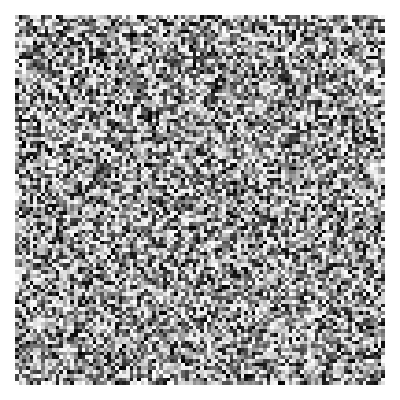
\includegraphics[width=.4\linewidth]{Images/gaussian_noise}
	}\qquad
	\subfloat[Perlin noise]{%
	\label{fig:perlin_noise}%
	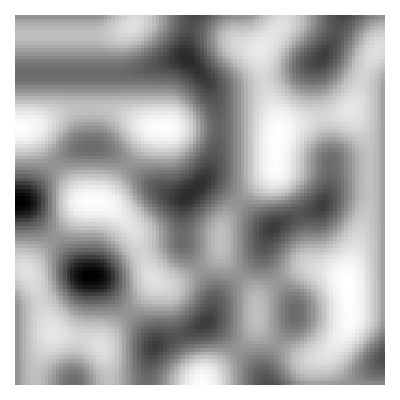
\includegraphics[width=.4\linewidth]{Images/perlin_noise}
	}
	\caption[Difference between noise patterns]{Difference between noise patterns.}
	\label{fig:noise_differences}
\end{figure}

\begin{figure}
	\centering
	\subfloat[Frequency 2]{%
	\label{fig:perlin_noise_2}%
	
\includegraphics[width=.3\linewidth]{Images/perlin_noise_2}
	}\quad
	\subfloat[Frequency 5]{%
	\label{fig:perlin_noise_5}%
	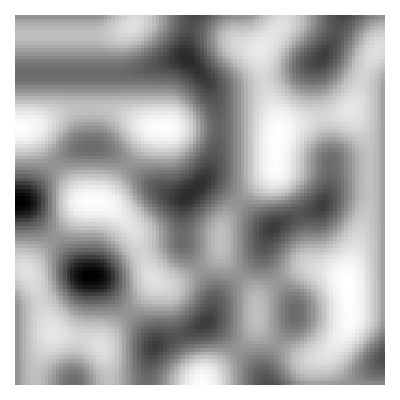
\includegraphics[width=.3\linewidth]{Images/perlin_noise}
	}\quad
	\subfloat[Frequency 20]{%
	\label{fig:perlin_noise_20}%
	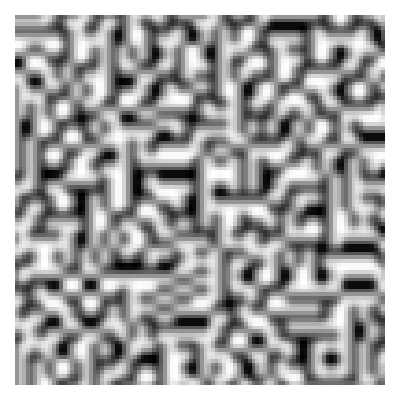
\includegraphics[width=.3\linewidth]{Images/perlin_noise_20}
	}
	\caption[Influence of frequency on Perlin noise]{Influence of frequency on Perlin noise patterns.}
	\label{fig:perlin_noise_frequencies}
\end{figure}

The second improvement is to use a regional mask. The original \gls{ba} applies a perturbation to the images as a whole. Every pixel will be perturbed with the same magnitude. This magnitude can be altered on a per-pixel basis when using a mask. Pixels that are further away from the target image will receive a larger perturbation than pixels that are already close to the corresponding pixel in the target. The mask $m$ is constructed according to equation \ref{eq:mask} based on the original image $x_{orig}$ and the adversarial image $x_{adv}$. It is then pixel-wise applied to the sampled perturbation in equation \ref{eq:mask_app}. The masked perturbation is normalized afterwards.\\ 

\begin{align}
m &= | x_{adv} - x_{orig}| \label{eq:mask}\\
\eta_{k} &= m \odot \eta_k; \eta_k = \frac{\eta_k}{\| \eta_k \|} \label{eq:mask_app}
\end{align}

This technique improves efficiency since the search space is significantly reduced. It is also possible to engineer masks for specific examples in order to incorporate other knowledge in the attack.\\

The final improvement is based on the idea of transfer attacks. A surrogate model is trained and will be used to calculate adversarial gradients. These gradients will then be used to bias the sampling direction for the orthogonal step. If the surrogate model does not closely resemble the defender, then the gradients will only hamper the speed of convergence of the attack instead of causing the attack to fail.

\begin{figure}
\centering
\tikzset{every picture/.style={line width=0.75pt}} %set default line width to 0.75pt        
\begin{tikzpicture}[x=0.75pt,y=0.75pt,yscale=-1,xscale=1]
%uncomment if require: \path (0,300); %set diagram left start at 0, and has height of 300

%Shape: Polygon Curved [id:ds5185908380685693] 
\draw  [fill={rgb, 255:red, 155; green, 155; blue, 155 }  ,fill opacity=0.5 ] (77.12,91.56) .. controls (95.12,69.56) and (136.12,35.56) .. (170.12,73.56) .. controls (204.12,111.56) and (165.12,154.56) .. (194.12,183.56) .. controls (223.12,212.56) and (189.12,259.56) .. (159.12,263.56) .. controls (129.12,267.56) and (33.12,279.56) .. (30.12,246.56) .. controls (27.12,213.56) and (79.12,216.56) .. (90.12,178.56) .. controls (101.12,140.56) and (59.12,113.56) .. (77.12,91.56) -- cycle ;
%Shape: Star [id:dp7170747564600322] 
\draw  [fill={rgb, 255:red, 0; green, 0; blue, 0 }  ,fill opacity=1 ] (122.62,191.06) -- (124.83,195.53) -- (129.76,196.24) -- (126.19,199.72) -- (127.03,204.63) -- (122.62,202.31) -- (118.22,204.63) -- (119.06,199.72) -- (115.49,196.24) -- (120.42,195.53) -- cycle ;
%Shape: Star [id:dp10477759386916752] 
\draw  [fill={rgb, 255:red, 0; green, 0; blue, 0 }  ,fill opacity=1 ] (94.62,14.06) -- (96.83,18.53) -- (101.76,19.24) -- (98.19,22.72) -- (99.03,27.63) -- (94.62,25.31) -- (90.22,27.63) -- (91.06,22.72) -- (87.49,19.24) -- (92.42,18.53) -- cycle ;
%Straight Lines [id:da2531323347021954] 
\draw    (94.62,21.56) -- (101.19,66.01) ;
\draw [shift={(101.62,68.98)}, rotate = 261.6] [fill={rgb, 255:red, 0; green, 0; blue, 0 }  ][line width=0.08]  [draw opacity=0] (8.93,-4.29) -- (0,0) -- (8.93,4.29) -- cycle    ;
%Straight Lines [id:da6594852147606747] 
\draw    (101.79,68.14) -- (91.03,74.6) ;
\draw [shift={(88.46,76.14)}, rotate = 329.04] [fill={rgb, 255:red, 0; green, 0; blue, 0 }  ][line width=0.08]  [draw opacity=0] (8.93,-4.29) -- (0,0) -- (8.93,4.29) -- cycle    ;
%Straight Lines [id:da6002841525279263] 
\draw    (88.46,76.14) -- (80.11,85.56) ;
\draw [shift={(78.12,87.81)}, rotate = 311.53] [fill={rgb, 255:red, 0; green, 0; blue, 0 }  ][line width=0.08]  [draw opacity=0] (8.93,-4.29) -- (0,0) -- (8.93,4.29) -- cycle    ;
%Straight Lines [id:da9148455444041863] 
\draw    (78.12,87.81) -- (71.8,97.16) ;
\draw [shift={(70.12,99.64)}, rotate = 304.06] [fill={rgb, 255:red, 0; green, 0; blue, 0 }  ][line width=0.08]  [draw opacity=0] (8.93,-4.29) -- (0,0) -- (8.93,4.29) -- cycle    ;
%Straight Lines [id:da47669503735159546] 
\draw    (70.12,99.64) -- (71.42,110.17) ;
\draw [shift={(71.79,113.14)}, rotate = 262.96] [fill={rgb, 255:red, 0; green, 0; blue, 0 }  ][line width=0.08]  [draw opacity=0] (8.93,-4.29) -- (0,0) -- (8.93,4.29) -- cycle    ;
%Straight Lines [id:da26104674623686774] 
\draw    (71.79,113.14) -- (76.37,123.08) ;
\draw [shift={(77.62,125.81)}, rotate = 245.27] [fill={rgb, 255:red, 0; green, 0; blue, 0 }  ][line width=0.08]  [draw opacity=0] (8.93,-4.29) -- (0,0) -- (8.93,4.29) -- cycle    ;
%Straight Lines [id:da9792015265988265] 
\draw    (77.62,125.81) -- (82.31,135.45) ;
\draw [shift={(83.62,138.14)}, rotate = 244.06] [fill={rgb, 255:red, 0; green, 0; blue, 0 }  ][line width=0.08]  [draw opacity=0] (8.93,-4.29) -- (0,0) -- (8.93,4.29) -- cycle    ;
%Straight Lines [id:da8018833944649997] 
\draw    (83.62,138.14) -- (87.84,148.69) ;
\draw [shift={(88.96,151.48)}, rotate = 248.2] [fill={rgb, 255:red, 0; green, 0; blue, 0 }  ][line width=0.08]  [draw opacity=0] (8.93,-4.29) -- (0,0) -- (8.93,4.29) -- cycle    ;
%Straight Lines [id:da7469050329272713] 
\draw    (88.96,151.48) -- (90.55,163.17) ;
\draw [shift={(90.96,166.14)}, rotate = 262.23] [fill={rgb, 255:red, 0; green, 0; blue, 0 }  ][line width=0.08]  [draw opacity=0] (8.93,-4.29) -- (0,0) -- (8.93,4.29) -- cycle    ;
%Straight Lines [id:da36931886382540347] 
\draw    (90.96,166.14) -- (88.57,177.7) ;
\draw [shift={(87.96,180.64)}, rotate = 281.69] [fill={rgb, 255:red, 0; green, 0; blue, 0 }  ][line width=0.08]  [draw opacity=0] (8.93,-4.29) -- (0,0) -- (8.93,4.29) -- cycle    ;
%Straight Lines [id:da3125285737899821] 
\draw    (87.96,180.64) -- (83.39,189.01) ;
\draw [shift={(81.96,191.64)}, rotate = 298.61] [fill={rgb, 255:red, 0; green, 0; blue, 0 }  ][line width=0.08]  [draw opacity=0] (8.93,-4.29) -- (0,0) -- (8.93,4.29) -- cycle    ;

%Curve Lines [id:da7332610230112269] 
\draw    (243,111.62) .. controls (297.92,70.43) and (367.93,279.11) .. (405,99.26) ;
%Shape: Star [id:dp6998768571531213] 
\draw  [fill={rgb, 255:red, 0; green, 0; blue, 0 }  ,fill opacity=1 ] (322.11,170.74) -- (325.14,176.87) -- (331.9,177.85) -- (327.01,182.62) -- (328.16,189.36) -- (322.11,186.18) -- (316.06,189.36) -- (317.22,182.62) -- (312.32,177.85) -- (319.09,176.87) -- cycle ;
%Straight Lines [id:da9467918607674688] 
\draw    (299.68,128.68) -- (331.29,83.87) ;
\draw [shift={(333.02,81.42)}, rotate = 125.2] [fill={rgb, 255:red, 0; green, 0; blue, 0 }  ][line width=0.08]  [draw opacity=0] (8.93,-4.29) -- (0,0) -- (8.93,4.29) -- cycle    ;
%Shape: Ellipse [id:dp07084957668985581] 
\draw  [color={rgb, 255:red, 128; green, 128; blue, 128 }  ,draw opacity=1 ][dash pattern={on 4.5pt off 4.5pt}] (264.94,181.03) .. controls (264.94,149.46) and (290.54,123.86) .. (322.11,123.86) .. controls (353.69,123.86) and (379.28,149.46) .. (379.28,181.03) .. controls (379.28,212.61) and (353.69,238.2) .. (322.11,238.2) .. controls (290.54,238.2) and (264.94,212.61) .. (264.94,181.03) -- cycle ;
%Straight Lines [id:da7547924674466151] 
\draw    (299.68,128.68) -- (326.52,124.97) ;
\draw [shift={(329.49,124.56)}, rotate = 172.13] [fill={rgb, 255:red, 0; green, 0; blue, 0 }  ][line width=0.08]  [draw opacity=0] (8.93,-4.29) -- (0,0) -- (8.93,4.29) -- cycle    ;
%Straight Lines [id:da7777022216727221] 
\draw    (329.49,124.56) -- (326.01,147.88) ;
\draw [shift={(325.57,150.85)}, rotate = 278.49] [fill={rgb, 255:red, 0; green, 0; blue, 0 }  ][line width=0.08]  [draw opacity=0] (8.93,-4.29) -- (0,0) -- (8.93,4.29) -- cycle    ;
%Straight Lines [id:da931484330606797] 
\draw [color={rgb, 255:red, 128; green, 128; blue, 128 }  ,draw opacity=1 ] [dash pattern={on 0.84pt off 2.51pt}]  (333.02,81.42) -- (329.49,124.56) ;


% Text Node
\draw (328.21,263) node   [align=left] {\begin{minipage}[lt]{96.27pt}\setlength\topsep{0pt}
classified correctly
\end{minipage}};
% Text Node
\draw (326.21,62) node   [align=left] {\begin{minipage}[lt]{96.27pt}\setlength\topsep{0pt}
classified incorrectly
\end{minipage}};
% Text Node
\draw (325.12,211.56) node   [align=left] {\begin{minipage}[lt]{68pt}\setlength\topsep{0pt}
original image
\end{minipage}};
% Text Node
\draw (112.21,256.14) node   [align=left] {\begin{minipage}[lt]{96.27pt}\setlength\topsep{0pt}
classified correctly
\end{minipage}};
% Text Node
\draw (106,13) node [anchor=north west][inner sep=0.75pt]   [align=left] {starting image};
% Text Node
\draw (56.21,116) node  [rotate=-286.01] [align=left] {\begin{minipage}[lt]{96.27pt}\setlength\topsep{0pt}
classified incorrectly
\end{minipage}};
% Text Node
\draw (120.12,225.56) node   [align=left] {\begin{minipage}[lt]{68pt}\setlength\topsep{0pt}
original image
\end{minipage}};
% Text Node
\draw (381.43,114.71) node   [align=left] {\begin{minipage}[lt]{68pt}\setlength\topsep{0pt}
1
\end{minipage}};
% Text Node
\draw (377.9,148.85) node   [align=left] {\begin{minipage}[lt]{68pt}\setlength\topsep{0pt}
2
\end{minipage}};
% Text Node
\draw (330,130) node [anchor=north west][inner sep=0.75pt]   [align=left] {$\displaystyle \epsilon $};
% Text Node
\draw (305,86) node [anchor=north west][inner sep=0.75pt]   [align=left] {$\displaystyle \eta $};


\end{tikzpicture}
\caption[Intuition of the Boundary Attack]{Intuition behind the Boundary Attack. On the left the path of the attack is shown. The first step is a projection onto the boundary, afterwards it follows the decision boundary of the class of the original image. Each arrow represents one iteration of the attack. On the right, the two different steps of each iteration can be seen. In the first step, a random direction is sampled and projected onto a sphere around the original image. The second step is to take a step towards the original image from this new position. Image inspired by \cite{boundary_attack}.}
\label{fig:boundary_attack_intuition}
\end{figure}

\section{HopSkipJumpAttack}
\gls{hsja} \cite{hsja}, like \gls{ba}, is a decision-based adversarial attack that starts from an adversarial input. The initial input is obtained in an identical manner as in \gls{ba}. \gls{hsja} is an iterative algorithm that consists of three steps.\\

The first step is a projection onto the decision boundary of the model under attack. This projection is carried out using a binary search. The second step is to estimate the direction of the gradient at the boundary. Different directions are sampled from a uniform distribution over a $d$-dimensional sphere, where $d$ is the input dimension. This random direction is added to the boundary point, generating a new query for the model. The results of these queries are combined to a gradient estimation~$\widetilde{\nabla S}$ using the Monte Carlo estimate of equation \ref{eq:monte_carlo_estimate}. In this equation $u_b$ are the random directions and $x_t$ is the boundary position. $B$ is the number of random directions that needs to be sampled. This number increases based on the current iteration of the attack to reduce the variance of the estimate. The function~$\phi_{x^*}$ returns 1 if the new position is adversarial and -1 if it is not adversarial. $\delta$ is a positive parameter determining the size of the $d$-dimensional sphere.

\begin{equation}\label{eq:monte_carlo_estimate}
\widetilde{\nabla S}(x_t,\delta) := \frac{1}{B} \sum_{b=1}^{B}\phi_{x^*}(x_t + \delta u_b)u_b
\end{equation}

Once the gradient has been estimated, the third and final operation is to take a step along this gradient. The step size is determined using a geometric progression scheme. These steps are iteratively repeated until the pre-set stopping criterion is met. Figure \ref{fig:hsja_intuition} represents the intuition behind \gls{hsja} in a graphical manner.\\

\gls{hsja} eclipses \gls{ba} and \gls{bba} both on median distance against queries and attack success rates using a limited amount of queries. The untargeted version of \gls{hsja} is able to compete with white box attacks on the ImageNet dataset \cite{imagenet}. It also performs similar or superior to white box attacks such as the C\&W attack \cite{cw_attack} when evaluated against defensive mechanisms such as defensive distillation \cite{defensive_distillation}, region-based classification \cite{region-based_classification} and adversarial training \cite{FGSM}.


\begin{figure}
\centering


\tikzset{every picture/.style={line width=0.75pt}} %set default line width to 0.75pt        

\begin{tikzpicture}[x=0.75pt,y=0.75pt,yscale=-1,xscale=1]
%uncomment if require: \path (0,300); %set diagram left start at 0, and has height of 300

%Curve Lines [id:da9704742483773781] 
\draw    (243,111.62) .. controls (297.92,70.43) and (367.93,279.11) .. (405,99.26) ;
%Shape: Star [id:dp26832364802919195] 
\draw  [fill={rgb, 255:red, 0; green, 0; blue, 0 }  ,fill opacity=1 ] (322.11,170.74) -- (325.14,176.87) -- (331.9,177.85) -- (327.01,182.62) -- (328.16,189.36) -- (322.11,186.18) -- (316.06,189.36) -- (317.22,182.62) -- (312.32,177.85) -- (319.09,176.87) -- cycle ;
%Shape: Ellipse [id:dp9511930412387599] 
\draw  [color={rgb, 255:red, 128; green, 128; blue, 128 }  ,draw opacity=1 ][dash pattern={on 4.5pt off 4.5pt}] (274.97,141.94) .. controls (274.97,120.26) and (292.54,102.69) .. (314.22,102.69) .. controls (335.9,102.69) and (353.48,120.26) .. (353.48,141.94) .. controls (353.48,163.63) and (335.9,181.2) .. (314.22,181.2) .. controls (292.54,181.2) and (274.97,163.63) .. (274.97,141.94) -- cycle ;
%Shape: Circle [id:dp5681517768642557] 
\draw  [fill={rgb, 255:red, 0; green, 0; blue, 0 }  ,fill opacity=1 ] (298,72.3) .. controls (298,71.03) and (299.03,70) .. (300.3,70) .. controls (301.57,70) and (302.6,71.03) .. (302.6,72.3) .. controls (302.6,73.57) and (301.57,74.6) .. (300.3,74.6) .. controls (299.03,74.6) and (298,73.57) .. (298,72.3) -- cycle ;
%Straight Lines [id:da06387380835189371] 
\draw    (300.3,72.3) -- (313.63,139) ;
\draw [shift={(314.22,141.94)}, rotate = 258.7] [fill={rgb, 255:red, 0; green, 0; blue, 0 }  ][line width=0.08]  [draw opacity=0] (8.93,-4.29) -- (0,0) -- (8.93,4.29) -- cycle    ;
%Straight Lines [id:da5011613685801404] 
\draw [color={rgb, 255:red, 155; green, 155; blue, 155 }  ,draw opacity=1 ][line width=0.75]  [dash pattern={on 0.84pt off 2.51pt}]  (314.22,141.94) -- (279.9,127.76) ;
\draw [shift={(278.05,127)}, rotate = 22.45] [fill={rgb, 255:red, 155; green, 155; blue, 155 }  ,fill opacity=1 ][line width=0.08]  [draw opacity=0] (12,-3) -- (0,0) -- (12,3) -- cycle    ;
%Shape: Boxed Line [id:dp5969211465757109] 
\draw [color={rgb, 255:red, 155; green, 155; blue, 155 }  ,draw opacity=1 ][line width=0.75]  [dash pattern={on 0.84pt off 2.51pt}]  (314.22,141.94) -- (327.54,107.28) ;
\draw [shift={(328.26,105.41)}, rotate = 111.02] [fill={rgb, 255:red, 155; green, 155; blue, 155 }  ,fill opacity=1 ][line width=0.08]  [draw opacity=0] (12,-3) -- (0,0) -- (12,3) -- cycle    ;
%Shape: Boxed Line [id:dp06580944891073615] 
\draw [color={rgb, 255:red, 155; green, 155; blue, 155 }  ,draw opacity=1 ][line width=0.75]  [dash pattern={on 0.84pt off 2.51pt}]  (314.22,141.94) -- (350.1,132.34) ;
\draw [shift={(352.03,131.82)}, rotate = 165.01] [fill={rgb, 255:red, 155; green, 155; blue, 155 }  ,fill opacity=1 ][line width=0.08]  [draw opacity=0] (12,-3) -- (0,0) -- (12,3) -- cycle    ;
%Shape: Boxed Line [id:dp5760742560965917] 
\draw [color={rgb, 255:red, 155; green, 155; blue, 155 }  ,draw opacity=1 ][line width=0.75]  [dash pattern={on 0.84pt off 2.51pt}]  (314.22,141.94) -- (340.03,168.65) ;
\draw [shift={(341.42,170.09)}, rotate = 225.98] [fill={rgb, 255:red, 155; green, 155; blue, 155 }  ,fill opacity=1 ][line width=0.08]  [draw opacity=0] (12,-3) -- (0,0) -- (12,3) -- cycle    ;
%Shape: Boxed Line [id:dp6962455418332032] 
\draw [color={rgb, 255:red, 155; green, 155; blue, 155 }  ,draw opacity=1 ][line width=0.75]  [dash pattern={on 0.84pt off 2.51pt}]  (314.22,141.94) -- (283.71,163.13) ;
\draw [shift={(282.07,164.27)}, rotate = 325.23] [fill={rgb, 255:red, 155; green, 155; blue, 155 }  ,fill opacity=1 ][line width=0.08]  [draw opacity=0] (12,-3) -- (0,0) -- (12,3) -- cycle    ;
%Straight Lines [id:da09211424476397356] 
\draw    (314.22,141.94) -- (345.36,106.42) ;
\draw [shift={(347.33,104.17)}, rotate = 131.23] [fill={rgb, 255:red, 0; green, 0; blue, 0 }  ][line width=0.08]  [draw opacity=0] (8.93,-4.29) -- (0,0) -- (8.93,4.29) -- cycle    ;
%Shape: Boxed Line [id:dp11391160549760482] 
\draw [color={rgb, 255:red, 155; green, 155; blue, 155 }  ,draw opacity=1 ][line width=0.75]  [dash pattern={on 0.84pt off 2.51pt}]  (314.22,141.94) -- (349.44,153.74) ;
\draw [shift={(351.34,154.37)}, rotate = 198.52] [fill={rgb, 255:red, 155; green, 155; blue, 155 }  ,fill opacity=1 ][line width=0.08]  [draw opacity=0] (12,-3) -- (0,0) -- (12,3) -- cycle    ;
%Shape: Boxed Line [id:dp7901030813069994] 
\draw [color={rgb, 255:red, 155; green, 155; blue, 155 }  ,draw opacity=1 ][line width=0.75]  [dash pattern={on 0.84pt off 2.51pt}]  (314.22,141.94) -- (302.05,106.86) ;
\draw [shift={(301.39,104.97)}, rotate = 70.87] [fill={rgb, 255:red, 155; green, 155; blue, 155 }  ,fill opacity=1 ][line width=0.08]  [draw opacity=0] (12,-3) -- (0,0) -- (12,3) -- cycle    ;
%Shape: Boxed Line [id:dp12912601709580973] 
\draw [color={rgb, 255:red, 155; green, 155; blue, 155 }  ,draw opacity=1 ][line width=0.75]  [dash pattern={on 0.84pt off 2.51pt}]  (314.22,141.94) -- (319.79,178.66) ;
\draw [shift={(320.09,180.64)}, rotate = 261.38] [fill={rgb, 255:red, 155; green, 155; blue, 155 }  ,fill opacity=1 ][line width=0.08]  [draw opacity=0] (12,-3) -- (0,0) -- (12,3) -- cycle    ;
%Shape: Boxed Line [id:dp15440737606551624] 
\draw [color={rgb, 255:red, 155; green, 155; blue, 155 }  ,draw opacity=1 ][line width=0.75]  [dash pattern={on 0.84pt off 2.51pt}]  (314.22,141.94) -- (301.49,176.83) ;
\draw [shift={(300.81,178.71)}, rotate = 290.05] [fill={rgb, 255:red, 155; green, 155; blue, 155 }  ,fill opacity=1 ][line width=0.08]  [draw opacity=0] (12,-3) -- (0,0) -- (12,3) -- cycle    ;
%Shape: Boxed Line [id:dp47011579703760575] 
\draw [color={rgb, 255:red, 155; green, 155; blue, 155 }  ,draw opacity=1 ][line width=0.75]  [dash pattern={on 0.84pt off 2.51pt}]  (314.22,141.94) -- (277.11,143.45) ;
\draw [shift={(275.11,143.53)}, rotate = 357.68] [fill={rgb, 255:red, 155; green, 155; blue, 155 }  ,fill opacity=1 ][line width=0.08]  [draw opacity=0] (12,-3) -- (0,0) -- (12,3) -- cycle    ;
%Shape: Boxed Line [id:dp3426945663084944] 
\draw [color={rgb, 255:red, 155; green, 155; blue, 155 }  ,draw opacity=1 ][line width=0.75]  [dash pattern={on 0.84pt off 2.51pt}]  (314.22,141.94) -- (345.13,121.35) ;
\draw [shift={(346.79,120.24)}, rotate = 146.33] [fill={rgb, 255:red, 155; green, 155; blue, 155 }  ,fill opacity=1 ][line width=0.08]  [draw opacity=0] (12,-3) -- (0,0) -- (12,3) -- cycle    ;

% Text Node
\draw (328.21,263) node   [align=left] {\begin{minipage}[lt]{96.27pt}\setlength\topsep{0pt}
classified correctly
\end{minipage}};
% Text Node
\draw (326.21,62) node   [align=left] {\begin{minipage}[lt]{96.27pt}\setlength\topsep{0pt}
classified incorrectly
\end{minipage}};
% Text Node
\draw (325.12,211.56) node   [align=left] {\begin{minipage}[lt]{68pt}\setlength\topsep{0pt}
original image
\end{minipage}};
% Text Node
\draw (304.6,75.3) node [anchor=north west][inner sep=0.75pt]   [align=left] {1};
% Text Node
\draw (262.33,131.33) node [anchor=north west][inner sep=0.75pt]   [align=left] {2};
% Text Node
\draw (346.33,92.67) node [anchor=north west][inner sep=0.75pt]   [align=left] {3};
\end{tikzpicture}
\caption[Intuition of the HopSkipJumpAttack]{Intuition behind the HopSkipJumpAttack. Each iteration consists of three steps. The first step is a projection onto the boundary. The second step is the estimation of the gradient at this point. This is done by sampling directions from a uniform distribution and querying the model under attack from this new position (grey arrows). The results are combined via the Monte Carlo estimate. The third and final step is to take a step along the estimated gradient. Image inspired by \cite{hsja}.}
\label{fig:hsja_intuition}
\end{figure}

\begin{figure}
\centering
\begin{tikzpicture}[xscale=0.75, yscale=0.75]
\definecolor{clr2}{RGB}{31,182,83}
\tikzset{
dot/.style = {circle, fill, minimum size=#1,
              inner sep=0pt, outer sep=0pt},
dot/.default = 6pt % size of the circle diameter 
}
\draw [fill={rgb, 255:red, 155; green, 155; blue, 155 }  ,fill opacity=0.5, draw=none] (0,7.5) -- (10,2.5) -- (10,10) -|cycle; % Fill above line

\path[name path=DB,draw, line width=0.5mm] (0,7.5) -- (10, 2.5); % Decision boundary

\begin{scope}[every node/.style={dot,thick,draw,anchor=base,fill=black}] % Circles
	\node[] (xo) at (3,3){}; %xo
	\node[] (xb) at (9,3){}; %xb
\end{scope}

\begin{scope}[red,line width=0.5mm]
\draw[] (xb) arc [
	start angle = 0,
	end angle = 180,
	radius = 3
];
\draw[] (xb) arc [
	start angle = 0,
	delta angle = -20,
	radius = 3
];
\draw[] (xo) arc [
	start angle = 180,
	delta angle = 20,
	radius = 3
];
\end{scope}

\begin{scope}[every node/.style={dot,thick,draw,anchor=base,fill=black}] % Circles
	\node[label=225:$x_o$] (xo) at (3,3){}; %xo
	\node[label=45:$x_b$] (xb) at (9,3){}; %xb
\end{scope}

\node[label=270:$u$] (xu) at (4.5,3){};
\node[label=180:$v$] (xv) at (3,4.5){};
\node[] (dl) at (3,1.5){};
\node[] (dr) at (9,1.5){};
\node[] (dal) at (3,0.5){};
\node[] (dar) at (7,0.5){};
\node[] (rpx) at (7,3){};
\path [-,line width=0.1mm, name path=guideline] (xo.east) edge (xb.west); % Guideline xo xb
\path [-latex, line width=0.5mm] (xo.east) edge (xu.west); % U arrow
\path [-latex, line width=0.5mm] (xo.north) edge (xv.south); % V arrow
\draw [spath/save=black, name path=blackarc, dashed] (rpx.center) arc (0:60:4);
\draw[dashed] (rpx) arc [start angle = 0, delta angle = -10, radius=4];
\path[spath/save=red, name path=redcircle] (xb) arc [
	start angle = 0,
	end angle = 180,
	radius = 3
];
\tikzset{
	spath/split at intersections={red}{black},
	spath/get components of ={black}\blackCpt,
}

\path[name intersections={of=DB and redcircle,by={Z, Z1}}];
\path [name intersections={of=blackarc and redcircle, by=intersect}];
\node[label=45:$z^*(\theta)$,dot,draw=red,anchor=base,fill=red] (i) at (intersect){};
\node[label=$z^*(\theta^*)$,dot,thick,draw=red,anchor=base,fill=red] (i2) at (Z1){};

\draw[spath/use={\getComponentOf\blackCpt{1}}, -latex, line width=0.5mm] node[right, pos=0.5] {$\theta$};
\path [dashed] (xo.center) edge (i.center);



\begin{scope}[color={rgb, 255:red, 31; green, 182; blue, 83}]
	\path [dashed] (dal.center) edge (xo.center);
	\path [dashed] (dr.center) edge (xb.center);
	\path [dashed] (dar.center) edge (rpx.center);
	\path [latex-latex, line width=0.5mm] (dl.center) edge node[fill=white] {$d$} (dr.center);
	\path [latex-latex, line width=0.5mm] (dal.center) edge node[fill=white] {$d(1-\alpha)$} (dar.center);
\end{scope}

\node[] (p) at (2,9){};
\draw [-latex, line width=0.5mm, blue, spath/save=normal] ($(xb)!(p)!(0,7.5)$) -- (p) node[]{$n$};
\draw [dashed, blue, line width=0.5mm] ($(xb)!(p)!(0,7.5)$) -- ($(xb)!(p)!(0,7.5) + (2,0)$);
\path[spath/save=dash] ($(xb)!(p)!(0,7.5) + (1.5,0)$) arc [start angle = 0, end angle = 90, radius = 1.5];
\tikzset{
	spath/split at intersections={normal}{dash},
	spath/get components of ={dash}\blueCpt,
}
\draw[spath/use={\getComponentOf\blueCpt{1}}, -latex, line width=0.5mm, blue] node[right, pos=0.5] {$\psi$};

\node[] at (8,9.5) {$\mathcal{O} \cap \mathcal{P}$};
\node[] (text) at (1,5.5) {$\partial\mathcal{O} \cap \mathcal{P}$};
\node[] (line) at (0.5,7.25) {};
\draw (text) to[out=0,in=-70] (line);
\end{tikzpicture}
\caption[Geographical configuration of SurFree]{•}
\label{fig:surfree}
\end{figure}


\section{Stateful defense}\label{sec:stateful_detection}
The defensive schemes discussed in section \ref{sec:adversarial_defenses} all operate on the query level. They try to detect and flag possible attacks based on a single query without taking other context into account. The stateful detection mechanism by Chen, Carlini and Wagner \cite{chen_stateful_2019} is different in this aspect. As the name suggests, it holds state of previously submitted queries. It is similar to the defenses that use proximity measurements, but the measurement is between queries instead of between the query and training data.\\

All queries submitted to the model equipped with a stateful detection mechanism are stored in a history buffer. Each user of the model has a distinct history buffer, where its queries are stored. These buffers can be bounded by time or number of queries depending on the resources available and the use case of the model. Each time a query is submitted to the model, the average distance to its $k$ nearest neighbors is calculated and if this distance is lower than a certain threshold, then the user gets flagged by the mechanism. Appropriate actions such as banning the account can be taken.\\

The distance metric is not calculated in input space. Each query is encoded by a deep similarity encoder \cite{deep_similarity_encoder} to an encoded space, typically of a lower dimension. In this encoded space, images which represent perceptually similar objects are clustered together. The advantage of the encoded space is twofold. Firstly, the dimension of the encoded space is smaller than the dimension of the input space. Therefore less space is needed to store the history buffers. Secondly, simpler distance metrics such as $L_2$-distance in input space can easily be evaded by an attacker. For example the $L_2$-distance can be significantly increased by simply rotating or shifting the input image.\\

The parameter $k$, the number of neighbors to consider is picked as follows. As the training data of the model consists of only benign queries, no attacks should be flagged when feeding the stateful detection mechanism with this data. To allow for some more leniency, a false positive rate of 0.1\% is still acceptable. For each value of $k$, a different threshold will be required to maintain the selected false positive rate. Larger values have the benefit of larger thresholds causing the defense to be more resilient, since attackers' images need to be more diverse. But $k$ is also the number of queries needed before an attack can be flagged. Therefore too large values for $k$ are disadvantageous. Smaller values also reduce computational cost. Chen, Carlini and Wagner set the value of $k$ to 50 for the CIFAR-10  dataset \cite{cifar}, since the thresholds increased sharply up to this value. Other datasets might require different values for $k$.

\section{PSO and distributed attacks}\label{sec:pso_and_distributed_attacks}
There have been several attempts to craft adversarial examples using an \gls{ea}. Previous attempts tried to reduce the number of queries needed to create a successful adversarial example by utilizing \glspl{ea} \cite{genattack,dong2019efficient,mosli2019they,audio_pso,distributed_pso_attack,suryanto2020}. \\

GenAttack \cite{genattack} and the similar efficient attack by Dong et al. \cite{dong2019efficient} use genetic algorithms in order to minimize the number of queries to the model. Both algorithms reduce the dimension of the search space to improve the efficiency of the attack. Once a promising perturbation is found in this lower dimensional space, it is upscaled using a bilinear transformation. By reducing the search space, the number of individuals in the genetic algorithm can be lowered, which in turn lowers the total amount of queries. GenAttack also uses annealing schemes to adaptively scale the parameters of the algorithm. This allows it to escape local optima and improve the adversarial example further. \\

AdversarialPSO \cite{mosli2019they} and the similar attack from \cite{audio_pso} use \gls{pso} as optimization routine on images and audio fragments respectively. Each particle represents a possible adversarial example. Both attacks use the standard rules of \gls{pso} as specified by \cite{pso} improved with a linearly decaying inertia weight \cite{inertia_weight}. The former attack also uses a constriction factor to avoid premature convergence \cite{constriction_factor}. While the latter solves this problem by generating new particles using a genetic algorithm when premature convergence is detected. Both algorithms rely on confidence scores to assign fitness values to certain positions in the search space. \gls{pso}-\gls{bba} \cite{distributed_pso_attack}, is similar to AdversarialPSO, but only relies on distances to determine fitness values. This attack can therefore also be used in decision-based settings instead of solely in score-based settings.\\

The idea behind the multi-group \gls{pso} attack \cite{suryanto2020} is to use multiple \gls{pso} swarms to escape local optima. The intuition behind it is inspired by the \gls{ddos} attack \cite{ddos}. The swarm is split into multiple smaller groups and each group is placed on a single node. The groups perform the standard \gls{pso} algorithm. The best position over all groups is communicated using a dedicated server. Each group submits its queries from its own node, tricking the defensive mechanism into thinking that multiple users are submitting queries. The authors state that this will ultimately result in less detections, but they have not evaluated this against a defensive scheme.\\

\chapter{Approach}\label{chap:approach}
The research concerning adversarial attacks and defenses is predominantly driven by a game of cat and mouse. Whenever a new attack is proposed, a defensive mechanism countering the novel attack is developed and vice versa. This work aims to create a new family of algorithms that can be used to perform both targeted and untargeted attacks. The goal of these algorithms is to craft adversarial examples comparable to state-of-the-art approaches while remaining undetected by the stateful detection mechanism \cite{chen_stateful_2019} described in section \ref{sec:stateful_detection}.

\section{Distribution}
The stateful detection mechanism \cite{chen_stateful_2019} assumes that queries can be traced back to their adversary and that there is no cooperation between different adversaries. This assumption can be problematic as $N$~collaborating adversaries can theoretically reduce the number of submitted queries per adversary by a factor of~$1/N$. Even a single adversary could set up multiple accounts and submit queries on each account until it is banned. Due to the reduced number of submitted queries, fewer attacks will be detected since each buffer of the defense mechanism only holds a fraction of all queries.\\

This work will aim to evade the detection mechanism by distributing the query submissions over multiple nodes. Each node will represent a different user of the model under attack. The users could theoretically be all different persons or they could be different accounts of the same person.\\

As described in section \ref{sec:pso_and_distributed_attacks}, several attempts have been made to distribute adversarial attacks \cite{distributed_pso_attack, suryanto2020}. However, none of these attacks have been evaluated against the stateful detection mechanism, since the goal of the distribution was to make the attack more efficient in terms of the distance between the original image and the resulting adversarial example. This work will distribute the query submission over multiple nodes in order to avoid detection.\\

\section{Optimization} \label{sec:optimization_approach}
As previously mentioned, reducing the number of submitted queries per adversary by a factor of~$1/N$, where $N$ is the number of collaborators, is straightforward. Adversaries can gain knowledge about the search space by cooperating with other adversaries. They can leverage this knowledge to reduce the number of submitted queries even more. This idea has been utilized by multiple algorithms that were mentioned in section \ref{sec:pso_and_distributed_attacks}. These algorithms used some form of \gls{pso} to optimize the final adversarial example. However all but the algorithm by Xiang et al \cite{distributed_pso_attack} rely on the confidence scores of the model for the fitness value calculation. All attacks discussed use \gls{pso} as an attack in itself. This work will combine the benefits of state-of-the-art black-box attacks and \gls{pso}.

\section{Problem statement}\label{sec:approach}
The remaining sections of this work will propose a new family of adversarial attacks. First, a threat model is defined in section \ref{sec:threat_model}. All remaining experiments will be performed with this threat model in mind. Afterwards, the novel adversarial algorithm is proposed in section \ref{sec:combining_pso_bba}. This algorithm is iteratively improved based on the results of the experiments. Finally, the final algorithm will be compared with the state-of-the-art decision-based attack in section \ref{sec:comparison}.\\

During the process of creating, improving and optimizing the attack, this work tries to answer the following research questions. 
\begin{itemize}
	\item What are the (dis)advantages of using \gls{pso} concerning vanilla adversarial attacks?
	\item How can \gls{pso} be combined with state-of-the-art adversarial attacks?
	\item What are the (dis)advantages of distributing an adversarial attack?
	\item How can adversarial attacks be made more evasive?
\end{itemize} 

\section{Threat model}\label{sec:threat_model}
This section will describe the threat model that will be used for the remainder of this work. The first and most impactful assumption is that the model under attack will only output labels for the input. There will be no confidence scores or model parameters available. The proposed attack will have to be decision-based. Most real-world \glspl{api} will only expose the final decision to the user, causing decision-based attacks to be the only viable option. Decision-based attacks are the most restricted type of attack. Therefore they can also be applied to score-based and white-box models without altering the attack.\\

The proposed attack will be a targeted attack, as it is the most relevant type from a security point of view. A targeted attack implementation can also easily be ported to an untargeted variant. This is done by running a targeted attack for every possible class and selecting the one closest to the original image.\\

The model will be defended by a stateful detection mechanism \cite{chen_stateful_2019} as described in section \ref{sec:stateful_detection}. It will have a query bounded buffer for each account. Once a query has been flagged as a potential attack, the account that submitted the query will be banned. The user will have to set up a fresh account to submit queries again. The model will track the IP addresses of the submitting users. This ensures that a banned user cannot sign into a fresh account and submit queries using the same banned machine.\\

There are two main fees associated with the model. The first fee is related to setting up an account. The assumption is made that setting up an account requires a valid credit card or phone number. Whenever an account is banned, the credit card or phone number is invalidated in the system, requiring the attacker to sign up for a new credit card or register for a new phone number. This cost is identical to the assumption made by Chen et al \cite{chen_stateful_2019}. The second fee is related to the number of queries submitted to the model. The more queries an attacker submits, the higher the total cost will be. Chen et al \cite{chen_stateful_2019} did not incorporate a cost per query, but most vision \glspl{api}, such as Google Cloud Vision \cite{google_pricing} and Amazon Rekognition \cite{amazon_pricing} use this type of fee. There is also a possibility that the fees are replaced by a rate limit, allowing a user to submit a fixed number of queries over a given period.\\

These fees ensure that attackers need to be both efficient and evasive in order to be successful. The evasiveness of the attack is correlated to the number of detections by the stateful defense mechanism. Each detection essentially means that the attacker has to set up a new account and pay the associated cost. To compare the efficiency of different attacks, every run of an attack has a budget of queries. The attack that has created an adversarial example closest to the original image inside this budget of queries, is the most efficient. The evasiveness of an attack is the primary concern since the cost of setting up a new account is significantly higher than the cost per query.


\chapter{Evaluation}
This chapter will discuss the experiments performed, as well as the ideas and intuitions behind them. The adversarial algorithm will be refined throughout the different subsections and the results of the refinement will be discussed at the end of each subsection.

\section{Evaluation protocol}
This subsection described the evaluation protocol that will be followed for all experiments performed. Experiments will be performed with the MNIST \cite{mnist} and CIFAR \cite{cifar} datasets. Some examples of these datasets are visualised in Figures \ref{fig:mnist} and \ref{fig:cifar} respectively. A black box model is trained using the training data of the respective dataset. The architectures of the models are identical to the ones used in \cite{cw_attack, defensive_distillation}. A summary of the two architectures can be found in Table \ref{tbl:architectures}. The training parameters are also identical to the ones used in \cite{cw_attack, defensive_distillation}. These models remain unchanged for all experiments.\\

The trained models are then used to classify all instances in the test set of their respective dataset. The incorrectly classified examples are filtered out of this set as they are essentially already adversarial. The remaining examples can be used for experiments. A list of experiments is generated based on the remaining examples. An experiment consists of an original image, a target label and starting position(s). All future refinements will therefore perform the same set of experiments in order to make the comparison more fair. All random effects present in the algorithm are seeded for the same purpose.\\

\begin{figure}
\centering
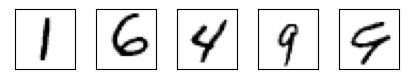
\includegraphics[width=\textwidth]{Images/mnist.png}
\caption[Some examples of the MNIST dataset]{Some examples of the MNIST dataset.}
\label{fig:mnist}
\end{figure}

\begin{figure}
\centering
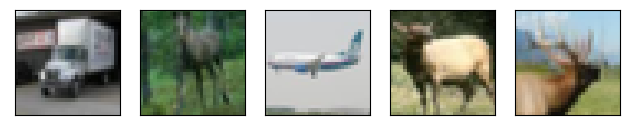
\includegraphics[width=\textwidth]{Images/cifar.png}
\caption[Some examples of the CIFAR-10 dataset]{Some examples of the CIFAR-10 dataset.}
\label{fig:cifar}
\end{figure}

\begin{table}
	\centering
	\caption[Model architectures for the MNIST and CIFAR model]{Model architectures for the MNIST and CIFAR models. The architectures are identical to \cite{cw_attack, defensive_distillation}.}
    \begin{tabular}{lll}\toprule
        Layer type     & MNIST Model &CIFAR Model\\ \midrule
		Convolution + \gls{relu}	&$3 \times 3 \times 32$ &$3\times3\times64$\\
		Convolution + \gls{relu}	&$3 \times 3 \times 32$ &$3\times3\times64$\\
		Max Pooling					&$2 \times2$			&$2\times2$\\
		Convolution + \gls{relu}	&$3 \times 3 \times 64$ &$3\times3\times128$\\
		Convolution + \gls{relu}	&$3 \times 3 \times 64$ &$3\times3\times128$\\
		Max Pooling					&$2 \times2$			&$2\times2$\\
		Fully Connected + \gls{relu}&200					&256\\
		Fully Connected + \gls{relu}&200					&256\\
		Softmax						&10						&10\\
        \bottomrule
    \end{tabular}
    \label{tbl:architectures}
\end{table}

The stateful defense mechanism \cite{chen_stateful_2019} will use a query bounded detector buffer of 1000 queries per user. The value of $k$ will be set to 50, as suggested by the authors of the paper. A threshold is determined in order to achieve a 0.1\% false positive detection rate on the training data. The detector buffer will be cleared after each detection to simulate the creation of a new account.\\

The algorithm receives a budget of \num{25000} queries to create an adversarial example. The final adversarial example will be evaluated on the $L_2$-distance to the original image and the total number of detections by the stateful defense mechanism.

\section{Determining the baseline}\label{sec:baseline}
The goal of this subsection is to determine a baseline to which all future algorithms will be compared. The baseline will be a vanilla \gls{bba} using the same hyperparameters as suggested in \cite{brunner_guessing_2019}. The orthogonal step will be set to 0.05 and the source step to 0.002. Both the Perlin noise improvement and the regional masking improvement will be used. No gradients of surrogate models will be calculated as the authors of the paper already mentioned that the improvement was marginal.\\

Table \ref{tbl:baseline} reports the average $L_2$-distance and the average number of detections for the different datasets. 

\begin{table}
	\centering
	\caption[Baseline results]{Results for the \gls{bba} baseline approach on MNIST and CIFAR-10 dataset.}
	\label{tbl:baseline}
	\begin{tabular}{lrrrr}\toprule
			& \multicolumn{2}{c}{MNIST} &\multicolumn{2}{c}{CIFAR} \\ \cmidrule(r){2-3} \cmidrule(r){4-5}
	Attack				&Distance	&Detections	&Distance	&Detections \\ \midrule
	Baseline \gls{bba}	&3.027		&339		&1.359			&475 \\ \bottomrule
	
	\end{tabular}
\end{table}

\section{Applying PSO to BBA} \label{sec:combining_pso_bba}
As mentioned in section \ref{sec:optimization_approach}, previous attempts to craft adversarial example using \gls{pso} used \gls{pso} to guide adversarial examples through the search space closer to the original image. This work aims to combine the benefits of \gls{pso} and an existing decision-based attack such as \gls{bba}.\\

Vanilla \gls{bba} has the disadvantage that, depending on the starting position, it might get trapped in a local optimum. By using \gls{pso} in combination with \gls{bba}, multiple starting positions can be explored and the probability of getting trapped is lowered. The intuition behind this idea is shown in Figure \ref{fig:applying_pso_to_bba}. The more starting positions there are, the higher the probability of finding the global optimum. There is however a clear trade-off in terms of efficiency. By having $n$ different starting positions, the query budget is essentially reduced by a factor~$n$ for each starting position.\\

The efficiency reduction does not have to pose a problem due to the implicit communication in the swarm. Particles can move to promising regions in the search space based on the information of their peers. The promising regions are therefore more queried.\\ 

The proposed \gls{pso}-\gls{bba} algorithm works as follows. Particles will perform a more aggressive version of \gls{bba}. The initial source step~$\epsilon$ is set significantly higher than in the vanilla version. The increased source step might cause the particle to end up in a non-adversarial decision region. Once this happens, the standard \gls{pso} equations (\ref{eq:velocity_update} and \ref{eq:position_update}) are used to guide the particle back to the adversarial region.\\

The inertia weight of the \gls{pso} equations is determined by the linearly decaying scheme of equation \ref{eq:weight}, with the weight decaying from 1 to 0. The acceleration coefficients $c$ are set based on an idea of multi-group \gls{pso}. Two groups with opposite acceleration coefficients are created. This approach helps escape local optima \cite{opposite_cs}. The equations for both $c_p$ and $c_g$ are:

\begin{align*}
c_p &= 
\begin{cases}
	\max(A1, A2), &\text{if } i\bmod 2 = 0\\
	\min(A1, A2), &\text{else}
\end{cases}\\
c_g &=
\begin{cases}
	\min(A1, A2), &\text{if } i\bmod 2 = 0\\
	\max(A1, A2), &\text{else}
\end{cases}\\
\end{align*} 

Here $i$ is the index of the particle in its swarm. The values of $A1$ and $A2$ are 1 and 2 respectively. These values are suggested by the authors of \cite{suryanto2020}.\\

The source step~$\epsilon$ will be changed after every iteration of the attack. Two separate multipliers are used to respectively increase and decrease the value of this parameter. The value of $\epsilon$ is slightly increased if the new position is still adversarial. Likewise it is decreased if the position is no longer adversarial.\\

By using \gls{pso} in combination with \gls{bba}, the advantage of multiple starting points, as explained in Figure \ref{fig:applying_pso_to_bba}, can be exploited, without having a less efficient attack as a whole. Whenever particles end up in non-adversarial regions, they will move closer to the best known position in the swarm due to the \gls{pso} equations. At then end of the attack, most particles will be in the same area of the search space, allowing for more exploitation in this specific area.\\

The \gls{pso} framework requires a fitness function the quantify the fitness of a position for the problem at hand. The authors of AdversarialPSO \cite{mosli2019they} suggested the following fitness function~$f$:

\begin{align}
	f(x) = |p_{x} - p_{x^{\prime}}| - \frac{c}{n}\|x-x^\prime\|_2   \label{eq:old_fitness}
\end{align}

Where $x$ is the position of the particle, $x^\prime$ is the original image, $p_{x}$ and $p_{x^\prime}$ are the confidence scores of the model in predicting the label of $x$ and $x^\prime$ respectively and $c$ is a constant to weight the penalty. However, as discussed in section \ref{sec:threat_model}, the confidence scores are not available for this specific attack. The fitness function in equation \ref{eq:old_fitness} also assumes that the position $x$ will always be adversarial. This will not be the case in the proposed algorithm. The fitness function will therefore be altered to the following:
\begin{align}
	f(x) = 
	\begin{cases}
 		\| x - x^\prime\|_2,	&\text{if } x \text{ is adversarial}\\
 		+\infty, 		& \text{else}
	\end{cases}
\end{align}

The infinite value for the fitness function inside non-adversarial decision regions acts as a penalty, causing the particles to quickly move out of these regions.\\

The same set of experiments as in section \ref{sec:baseline} has been performed. The experiments have been done using attacks with both five and ten particles. The initial step sizes have been set to 0.25 and 0.20 for MNIST and CIFAR respectively. The values for the increasing and decreasing multiplier have been set to 1.05 and 0.99 for both datasets. The results of the experiments can be found in Table \ref{tbl:pso_bba}.\\

The \gls{pso}-\gls{bba} algorithm outperforms the baseline in terms of distance to the original image, except for the ten particle version on the CIFAR dataset. The high number of particles requires sufficient queries in the beginning of the attack in order to discover promising regions in the high dimensional search space of CIFAR. The number of detections is lower for all variants of \gls{pso}-\gls{bba}. The different starting points have the added advantage that initial queries are more spread out over the search space. These queries are therefore less similar and the detector will not flag as much attacks. This effect can be seen in Figure \ref{fig:detections_bba_vs_pso_bba} for one experiment.\\

The number of detections drops as the number of particles increases. This was to be expected from the intuition behind \gls{pso}-\gls{bba}. However, the average $L_2$-distance to the original image is higher is higher for ten particles compared to five. To reduce the number of different parameters in future refinements, only swarms with five particles will be considered from here on.\\ 

\begin{figure}
	\centering
\tikzset{every picture/.style={line width=0.75pt}} %set default line width to 0.75pt        

\begin{tikzpicture}[x=0.75pt,y=0.75pt,yscale=-1,xscale=1]
%uncomment if require: \path (0,300); %set diagram left start at 0, and has height of 300

%Shape: Polygon Curved [id:ds39418321723754923] 
\draw  [fill={rgb, 255:red, 155; green, 155; blue, 155 }  ,fill opacity=0.5 ] (365.12,90.5) .. controls (383.12,68.5) and (424.12,34.5) .. (458.12,72.5) .. controls (492.12,110.5) and (453.12,153.5) .. (482.12,182.5) .. controls (511.12,211.5) and (477.12,258.5) .. (447.12,262.5) .. controls (417.12,266.5) and (321.12,278.5) .. (318.12,245.5) .. controls (315.12,212.5) and (367.12,215.5) .. (378.12,177.5) .. controls (389.12,139.5) and (347.12,112.5) .. (365.12,90.5) -- cycle ;
%Shape: Star [id:dp17995230177708343] 
\draw  [fill={rgb, 255:red, 0; green, 0; blue, 0 }  ,fill opacity=1 ] (410.62,190) -- (412.83,194.47) -- (417.76,195.18) -- (414.19,198.66) -- (415.03,203.57) -- (410.62,201.25) -- (406.22,203.57) -- (407.06,198.66) -- (403.49,195.18) -- (408.42,194.47) -- cycle ;
%Shape: Star [id:dp263511542953333] 
\draw  [fill={rgb, 255:red, 0; green, 0; blue, 0 }  ,fill opacity=1 ] (382.62,13) -- (384.83,17.47) -- (389.76,18.18) -- (386.19,21.66) -- (387.03,26.57) -- (382.62,24.25) -- (378.22,26.57) -- (379.06,21.66) -- (375.49,18.18) -- (380.42,17.47) -- cycle ;
%Straight Lines [id:da12241666866362477] 
\draw    (382.62,20.5) -- (389.19,64.95) ;
\draw [shift={(389.62,67.92)}, rotate = 261.6] [fill={rgb, 255:red, 0; green, 0; blue, 0 }  ][line width=0.08]  [draw opacity=0] (8.93,-4.29) -- (0,0) -- (8.93,4.29) -- cycle    ;
%Straight Lines [id:da7985170559413728] 
\draw    (389.79,67.08) -- (379.03,73.54) ;
\draw [shift={(376.46,75.08)}, rotate = 329.04] [fill={rgb, 255:red, 0; green, 0; blue, 0 }  ][line width=0.08]  [draw opacity=0] (8.93,-4.29) -- (0,0) -- (8.93,4.29) -- cycle    ;
%Straight Lines [id:da5286207592270582] 
\draw    (376.46,75.08) -- (368.11,84.5) ;
\draw [shift={(366.12,86.75)}, rotate = 311.53] [fill={rgb, 255:red, 0; green, 0; blue, 0 }  ][line width=0.08]  [draw opacity=0] (8.93,-4.29) -- (0,0) -- (8.93,4.29) -- cycle    ;
%Straight Lines [id:da4098354744836743] 
\draw    (366.12,86.75) -- (359.8,96.1) ;
\draw [shift={(358.12,98.58)}, rotate = 304.06] [fill={rgb, 255:red, 0; green, 0; blue, 0 }  ][line width=0.08]  [draw opacity=0] (8.93,-4.29) -- (0,0) -- (8.93,4.29) -- cycle    ;
%Straight Lines [id:da7402027038712158] 
\draw    (358.12,98.58) -- (359.42,109.11) ;
\draw [shift={(359.79,112.08)}, rotate = 262.96] [fill={rgb, 255:red, 0; green, 0; blue, 0 }  ][line width=0.08]  [draw opacity=0] (8.93,-4.29) -- (0,0) -- (8.93,4.29) -- cycle    ;
%Straight Lines [id:da22742294505428506] 
\draw    (359.79,112.08) -- (364.37,122.03) ;
\draw [shift={(365.62,124.75)}, rotate = 245.27] [fill={rgb, 255:red, 0; green, 0; blue, 0 }  ][line width=0.08]  [draw opacity=0] (8.93,-4.29) -- (0,0) -- (8.93,4.29) -- cycle    ;
%Shape: Boxed Line [id:dp17555971988752717] 
\draw    (362.2,200.74) -- (368.55,193.64) ;
\draw [shift={(370.55,191.4)}, rotate = 131.8] [fill={rgb, 255:red, 0; green, 0; blue, 0 }  ][line width=0.08]  [draw opacity=0] (8.93,-4.29) -- (0,0) -- (8.93,4.29) -- cycle    ;
%Shape: Star [id:dp5469311004467188] 
\draw  [fill={rgb, 255:red, 0; green, 0; blue, 0 }  ,fill opacity=1 ] (533.42,103.8) -- (535.63,108.27) -- (540.56,108.98) -- (536.99,112.46) -- (537.83,117.37) -- (533.42,115.05) -- (529.02,117.37) -- (529.86,112.46) -- (526.29,108.98) -- (531.22,108.27) -- cycle ;
%Shape: Star [id:dp8199494411723183] 
\draw  [fill={rgb, 255:red, 0; green, 0; blue, 0 }  ,fill opacity=1 ] (525,239.51) -- (527.2,243.97) -- (532.13,244.69) -- (528.57,248.17) -- (529.41,253.07) -- (525,250.76) -- (520.59,253.07) -- (521.43,248.17) -- (517.87,244.69) -- (522.8,243.97) -- cycle ;
%Shape: Star [id:dp3621439940158031] 
\draw  [fill={rgb, 255:red, 0; green, 0; blue, 0 }  ,fill opacity=1 ] (324.22,281.14) -- (326.43,285.61) -- (331.36,286.32) -- (327.79,289.8) -- (328.63,294.71) -- (324.22,292.39) -- (319.82,294.71) -- (320.66,289.8) -- (317.09,286.32) -- (322.02,285.61) -- cycle ;
%Shape: Star [id:dp886425904787334] 
\draw  [fill={rgb, 255:red, 0; green, 0; blue, 0 }  ,fill opacity=1 ] (298.22,198.74) -- (300.43,203.21) -- (305.36,203.92) -- (301.79,207.4) -- (302.63,212.31) -- (298.22,209.99) -- (293.82,212.31) -- (294.66,207.4) -- (291.09,203.92) -- (296.02,203.21) -- cycle ;
%Straight Lines [id:da29737150039250193] 
\draw    (533.42,111.3) -- (473.43,154.98) ;
\draw [shift={(471,156.74)}, rotate = 323.95] [fill={rgb, 255:red, 0; green, 0; blue, 0 }  ][line width=0.08]  [draw opacity=0] (8.93,-4.29) -- (0,0) -- (8.93,4.29) -- cycle    ;
%Straight Lines [id:da564242749820822] 
\draw    (298.22,206.24) -- (359.21,201) ;
\draw [shift={(362.2,200.74)}, rotate = 175.09] [fill={rgb, 255:red, 0; green, 0; blue, 0 }  ][line width=0.08]  [draw opacity=0] (8.93,-4.29) -- (0,0) -- (8.93,4.29) -- cycle    ;
%Straight Lines [id:da8824188996602935] 
\draw    (525,247.01) -- (490.26,231.18) ;
\draw [shift={(487.53,229.94)}, rotate = 24.49] [fill={rgb, 255:red, 0; green, 0; blue, 0 }  ][line width=0.08]  [draw opacity=0] (8.93,-4.29) -- (0,0) -- (8.93,4.29) -- cycle    ;
%Straight Lines [id:da172043009485096] 
\draw    (324.22,288.64) -- (343.77,267.35) ;
\draw [shift={(345.8,265.14)}, rotate = 132.55] [fill={rgb, 255:red, 0; green, 0; blue, 0 }  ][line width=0.08]  [draw opacity=0] (8.93,-4.29) -- (0,0) -- (8.93,4.29) -- cycle    ;
%Shape: Boxed Line [id:dp5913488094519332] 
\draw    (370.55,191.4) -- (374.75,182.84) ;
\draw [shift={(376.07,180.15)}, rotate = 116.11] [fill={rgb, 255:red, 0; green, 0; blue, 0 }  ][line width=0.08]  [draw opacity=0] (8.93,-4.29) -- (0,0) -- (8.93,4.29) -- cycle    ;
%Shape: Boxed Line [id:dp8616221435272089] 
\draw    (487.53,229.94) -- (491.55,221.3) ;
\draw [shift={(492.81,218.58)}, rotate = 114.93] [fill={rgb, 255:red, 0; green, 0; blue, 0 }  ][line width=0.08]  [draw opacity=0] (8.93,-4.29) -- (0,0) -- (8.93,4.29) -- cycle    ;
%Shape: Boxed Line [id:dp5796326247856174] 
\draw    (492.81,218.58) -- (494.7,209.24) ;
\draw [shift={(495.29,206.29)}, rotate = 101.39] [fill={rgb, 255:red, 0; green, 0; blue, 0 }  ][line width=0.08]  [draw opacity=0] (8.93,-4.29) -- (0,0) -- (8.93,4.29) -- cycle    ;
%Shape: Boxed Line [id:dp044334919963415986] 
\draw    (495.29,206.29) -- (492.57,197.16) ;
\draw [shift={(491.71,194.29)}, rotate = 73.42] [fill={rgb, 255:red, 0; green, 0; blue, 0 }  ][line width=0.08]  [draw opacity=0] (8.93,-4.29) -- (0,0) -- (8.93,4.29) -- cycle    ;
%Shape: Boxed Line [id:dp4387546700476397] 
\draw    (491.71,194.29) -- (486.61,186.24) ;
\draw [shift={(485,183.71)}, rotate = 57.58] [fill={rgb, 255:red, 0; green, 0; blue, 0 }  ][line width=0.08]  [draw opacity=0] (8.93,-4.29) -- (0,0) -- (8.93,4.29) -- cycle    ;
%Shape: Boxed Line [id:dp8947094222533136] 
\draw    (485,183.71) -- (478.98,176.32) ;
\draw [shift={(477.09,173.99)}, rotate = 50.85] [fill={rgb, 255:red, 0; green, 0; blue, 0 }  ][line width=0.08]  [draw opacity=0] (8.93,-4.29) -- (0,0) -- (8.93,4.29) -- cycle    ;
%Shape: Boxed Line [id:dp8126738394252795] 
\draw    (471,156.74) -- (473.27,166) ;
\draw [shift={(473.99,168.91)}, rotate = 256.19] [fill={rgb, 255:red, 0; green, 0; blue, 0 }  ][line width=0.08]  [draw opacity=0] (8.93,-4.29) -- (0,0) -- (8.93,4.29) -- cycle    ;
%Shape: Boxed Line [id:dp14754319972001273] 
\draw    (345.8,265.14) -- (355.11,267.18) ;
\draw [shift={(358.04,267.82)}, rotate = 192.33] [fill={rgb, 255:red, 0; green, 0; blue, 0 }  ][line width=0.08]  [draw opacity=0] (8.93,-4.29) -- (0,0) -- (8.93,4.29) -- cycle    ;
%Shape: Boxed Line [id:dp8374639915608668] 
\draw    (358.04,267.82) -- (367.46,269.26) ;
\draw [shift={(370.43,269.71)}, rotate = 188.71] [fill={rgb, 255:red, 0; green, 0; blue, 0 }  ][line width=0.08]  [draw opacity=0] (8.93,-4.29) -- (0,0) -- (8.93,4.29) -- cycle    ;
%Shape: Boxed Line [id:dp496623104677657] 
\draw    (370.43,269.71) -- (379.95,269.39) ;
\draw [shift={(382.95,269.29)}, rotate = 178.04] [fill={rgb, 255:red, 0; green, 0; blue, 0 }  ][line width=0.08]  [draw opacity=0] (8.93,-4.29) -- (0,0) -- (8.93,4.29) -- cycle    ;
%Shape: Boxed Line [id:dp34473561543285314] 
\draw    (382.95,269.29) -- (392.47,268.77) ;
\draw [shift={(395.46,268.61)}, rotate = 176.92] [fill={rgb, 255:red, 0; green, 0; blue, 0 }  ][line width=0.08]  [draw opacity=0] (8.93,-4.29) -- (0,0) -- (8.93,4.29) -- cycle    ;
%Shape: Boxed Line [id:dp22829712791209555] 
\draw    (395.46,268.61) -- (404.98,268.23) ;
\draw [shift={(407.98,268.11)}, rotate = 177.71] [fill={rgb, 255:red, 0; green, 0; blue, 0 }  ][line width=0.08]  [draw opacity=0] (8.93,-4.29) -- (0,0) -- (8.93,4.29) -- cycle    ;

%Shape: Polygon Curved [id:ds013419098702227128] 
\draw  [fill={rgb, 255:red, 155; green, 155; blue, 155 }  ,fill opacity=0.5 ] (72.05,88.7) .. controls (90.05,66.7) and (131.05,32.7) .. (165.05,70.7) .. controls (199.05,108.7) and (160.05,151.7) .. (189.05,180.7) .. controls (218.05,209.7) and (184.05,256.7) .. (154.05,260.7) .. controls (124.05,264.7) and (28.05,276.7) .. (25.05,243.7) .. controls (22.05,210.7) and (74.05,213.7) .. (85.05,175.7) .. controls (96.05,137.7) and (54.05,110.7) .. (72.05,88.7) -- cycle ;
%Shape: Star [id:dp9534459695500062] 
\draw  [fill={rgb, 255:red, 0; green, 0; blue, 0 }  ,fill opacity=1 ] (117.55,188.2) -- (119.76,192.67) -- (124.68,193.38) -- (121.12,196.86) -- (121.96,201.77) -- (117.55,199.45) -- (113.14,201.77) -- (113.99,196.86) -- (110.42,193.38) -- (115.35,192.67) -- cycle ;
%Shape: Star [id:dp3150974101447812] 
\draw  [fill={rgb, 255:red, 0; green, 0; blue, 0 }  ,fill opacity=1 ] (231.93,237.71) -- (234.13,242.17) -- (239.06,242.89) -- (235.49,246.37) -- (236.34,251.28) -- (231.93,248.96) -- (227.52,251.28) -- (228.36,246.37) -- (224.79,242.89) -- (229.72,242.17) -- cycle ;
%Straight Lines [id:da8721626382201679] 
\draw    (231.93,245.21) -- (197.19,229.38) ;
\draw [shift={(194.46,228.14)}, rotate = 24.49] [fill={rgb, 255:red, 0; green, 0; blue, 0 }  ][line width=0.08]  [draw opacity=0] (8.93,-4.29) -- (0,0) -- (8.93,4.29) -- cycle    ;
%Shape: Boxed Line [id:dp35233924811215767] 
\draw    (194.46,228.14) -- (198.48,219.5) ;
\draw [shift={(199.74,216.78)}, rotate = 114.93] [fill={rgb, 255:red, 0; green, 0; blue, 0 }  ][line width=0.08]  [draw opacity=0] (8.93,-4.29) -- (0,0) -- (8.93,4.29) -- cycle    ;
%Shape: Boxed Line [id:dp47377705399021885] 
\draw    (199.74,216.78) -- (201.62,207.44) ;
\draw [shift={(202.22,204.5)}, rotate = 101.39] [fill={rgb, 255:red, 0; green, 0; blue, 0 }  ][line width=0.08]  [draw opacity=0] (8.93,-4.29) -- (0,0) -- (8.93,4.29) -- cycle    ;
%Shape: Boxed Line [id:dp01327277725498055] 
\draw    (202.22,204.5) -- (199.5,195.36) ;
\draw [shift={(198.64,192.49)}, rotate = 73.42] [fill={rgb, 255:red, 0; green, 0; blue, 0 }  ][line width=0.08]  [draw opacity=0] (8.93,-4.29) -- (0,0) -- (8.93,4.29) -- cycle    ;
%Shape: Boxed Line [id:dp6860848467619505] 
\draw    (198.64,192.49) -- (193.53,184.44) ;
\draw [shift={(191.92,181.91)}, rotate = 57.58] [fill={rgb, 255:red, 0; green, 0; blue, 0 }  ][line width=0.08]  [draw opacity=0] (8.93,-4.29) -- (0,0) -- (8.93,4.29) -- cycle    ;
%Shape: Boxed Line [id:dp2849658598230065] 
\draw    (191.92,181.91) -- (185.91,174.52) ;
\draw [shift={(184.01,172.19)}, rotate = 50.85] [fill={rgb, 255:red, 0; green, 0; blue, 0 }  ][line width=0.08]  [draw opacity=0] (8.93,-4.29) -- (0,0) -- (8.93,4.29) -- cycle    ;


% Text Node
\draw (107.14,250.13) node   [align=left] {\begin{minipage}[lt]{96.27pt}\setlength\topsep{0pt}
classified correctly
\end{minipage}};
% Text Node
\draw (51.61,113.14) node  [rotate=-286.01] [align=left] {\begin{minipage}[lt]{96.27pt}\setlength\topsep{0pt}
classified incorrectly
\end{minipage}};
% Text Node
\draw (119.05,223.33) node   [align=left] {\begin{minipage}[lt]{68pt}\setlength\topsep{0pt}
original image
\end{minipage}};
% Text Node
\draw (400.21,251.93) node   [align=left] {\begin{minipage}[lt]{96.27pt}\setlength\topsep{0pt}
classified correctly
\end{minipage}};
% Text Node
\draw (344.71,114.94) node  [rotate=-286.01] [align=left] {\begin{minipage}[lt]{96.27pt}\setlength\topsep{0pt}
classified incorrectly
\end{minipage}};
% Text Node
\draw (412.12,225.13) node   [align=left] {\begin{minipage}[lt]{68pt}\setlength\topsep{0pt}
original image
\end{minipage}};


\end{tikzpicture}	
\caption[Intuition of multiple starting points]{The vanilla version of \gls{bba} might get stuck in a local optimum depending on the starting point (left plot). By starting from multiple positions, the probability that \gls{bba} gets stuck in a local optimum is reduced (right plot). The multiple starting points are particles in a \gls{pso} swarm.}
\label{fig:applying_pso_to_bba}
\end{figure}

\begin{figure}
\centering
\begin{tikzpicture}
\begin{axis}[width=12cm, height=5cm, xmin=0,xmax=25000, xlabel=Calls, ylabel=Detections, tick label style={/pgf/number format/fixed}, scaled ticks=false, enlarge x limits=0.01, xtick={0,5000,10000,15000,20000,25000},legend pos=north west,	legend style={draw=none},]
\addplot table[col sep=comma,x index=1,y expr=\thisrowno{0} + 1,mark=none] {Data/detections_bba.csv};
\addlegendentry{\gls{bba}};
\addplot table[col sep=comma,x index=1,y expr=\thisrowno{0} + 1,mark=none] {Data/detections_pso_bba.csv};
\addlegendentry{\gls{pso}-\gls{bba}};

\end{axis}
\end{tikzpicture}
\caption[Detections of the different attacks]{The cumulative number of detections for different attack algorithms for one specific MNIST experiment. The number of detections of the \gls{bba} algorithm steadily increases with the number of calls. The number of detections of the \gls{pso}-\gls{bba} algorithm increases more slowly in the beginning due to the dispersed nature of the attack. The increase is more sharp near the end of the attack.}
\label{fig:detections_bba_vs_pso_bba}
\end{figure}

\begin{table}
	\centering
	\caption[PSO-BBA results]{Results for the \gls{pso}-\gls{bba} approach on MNIST and CIFAR-10 dataset.}
	\label{tbl:pso_bba}
	\begin{tabular}{lrrrr}\toprule
			& \multicolumn{2}{c}{MNIST} &\multicolumn{2}{c}{CIFAR} \\ \cmidrule(r){2-3} \cmidrule(r){4-5}
	Attack				&Distance	&Detections	&Distance	&Detections \\ \midrule
	Baseline \gls{bba}	&3.027		&339		&1.359			&475 \\
	\gls{pso}-\gls{bba} (5 particles)	&2.691			&173			&1.133				&301 \\ 
	\gls{pso}-\gls{bba} (10 particles)	&2.788			&107			&1.782				&243 \\
	\bottomrule
	
	\end{tabular}
\end{table}

\section{Towards distribution of the attack}
The stateful defense mechanism \cite{chen_stateful_2019} makes the assumption that there is no collaboration between adversaries. Based on this assumption, each account or user will have its own detector buffer. This subsection aims to exploit this assumption by distributing the query submission over multiple accounts.\\

By distributing the query submissions over multiple accounts, the number of total detection should be reduced compared to \gls{bba} due to two reasons. The first reason is obvious. If a budget of \num{25000} queries is distributed over $N$ accounts, then every account will submit \num{25000} / $N$ queries. The less queries there are submitted, the less potential attacks will be detected. The second reason is due to \gls{pso}. As stated before, the different particles reside in different parts of the search space. This means that a detector buffer of a specific account will contain queries from all over the search space, causing the inter query distances to be larger. The latter reason was also present in the algorithm described in section \ref{sec:combining_pso_bba}.\\

It should be noted that there is only distribution at the query submission level. The algorithm itself will be executed on one machine without the need for distribution. Even the query submission can be done from one machine by constantly changing the \gls{api} key or by logging in and out of a specific account whenever it is needed. This approach makes the assumption that the \gls{api} under attack does not track the IP~address of the machine that submitted the query. Multiple machines might therefore be more convenient in a real attack setting.\\

This work simulates the multiple machines setting by having separate node (or machine) objects on the same machine. Instead of having a detector buffer for each node at the location of the model, the responsibility is moved upstream to the nodes themselves. Each node will have a buffer to which the query will be added. All queries will be passed to the model afterwards. In Figure \ref{fig:distribution_overview}, the distribution is shown schematically. 

\begin{figure}
\centering
\begin{tikzpicture}
\begin{scope}[every node/.style={rectangle,thick,draw,anchor=base, minimum width=20mm}]
	\node[align=center] (N1) at (3,5) {Node 1};
	\node[align=center] (N2) at (3,4) {Node 2};
	\node[align=center] (N3) at (3,3) {Node 3};
	\node[align=center] (NN) at (3,1) {Node $N$};
\end{scope}

\node[align=center,anchor=base, minimum width=20mm,rectangle] (N) at (3,2) {$\ldots$};

\begin{scope}[every node/.style={rectangle,thick,draw,anchor=base,minimum width=20mm, minimum height=10mm}]
	\node[align=right, left= 35mm of N3] (A) {Algorithm};
	\node[align=left, right= 35mm of N3] (M) {Model};
\end{scope}

\begin{scope}[]
	\path [->] (A.east) edge (N1.west);
	\path [->] (A.east) edge (N2.west);
	\path [->] (A.east) edge (N3.west);
%	\path [->] (A.east) edge (N.west);
	\path [->] (A.east) edge (NN.west);

	\path [->] (N1.east) edge (M.west);
	\path [->] (N2.east) edge (M.west);
	\path [->] (N3.east) edge (M.west);
%	\path [->] (N.east) edge (M.west);
	\path [->] (NN.east) edge (M.west);	
\end{scope}
\end{tikzpicture}
\caption[Schematic overview of the query submission distribution]{Schematic overview of the query submission distribution. Each arrow represents a query. The algorithm distributes the queries over the different nodes. Every node forwards its received queries to the model using the corresponding account. In a real setting, the model will have a detector buffer for every account. In this work the buffers are located on the nodes themselves.}
\label{fig:distribution_overview}
\end{figure}

\section{Throwing the defense off the scent}

\section{Optimizing the attack}

\chapter{Conclusion}\label{chap:conclusion}
%This chapter aims to conclude this work by answering the research questions posed in section \ref{sec:approach}:\\
%
%\textbf{What are the (dis)advantages of using \gls{pso} in relation to vanilla adversarial attacks?}\\
%\gls{pso} is an optimization framework where particles move through search space where every position is mapped to a fitness value. The framework tries to guide the particles to regions with good fitness values. \gls{pso} requires no notion of the underlying problem it is trying to solve. It only requires a fitness function to be defined for the entire search space. This allows for the optimization of problems that could not be solved analytically.\\
%
%Adversarial attacks can be seen as such a problem. It requires finding a position (or image) in search space that is as close as possible to an original image, while receiving a different classification than the original image by the model under attack. Depending on the information available about the model, white-box and black-box attacks can be distinguished. White-box attacks have complete knowledge about the model. This knowledge includes the architecture, parameters, weights and gradients. Especially the gradients are very useful in order to optimize the adversarial examples generated by an attack. Methods such as \gls{fgsm} \cite{FGSM} use these gradients to quickly improve the adversarial position. Whenever this information is available, \gls{pso} is not strong candidate for the optimization process as it does not use this information.\\
%
%However, most real models operate without providing this information to its users. Black-box attacks such as \gls{bba} \cite{brunner_guessing_2019} and \gls{hsja} \cite{hsja} are able to work around this lack of knowledge. \gls{hsja} in particular is able to closely match the performance of some white-box attacks, but it requires more queries in doing so. These extra queries allow for more detections by a stateful defense \cite{chen_stateful_2019}, since successive queries tend to be similar in appearance.\\
%
%\gls{pso} is less prone to detections due to its multiple starting points. The queries submitted to the model originate from different regions of the search space, making them less similar to each other. This is one of the main advantages of \gls{pso} as was discussed in section \ref{sec:combining_pso_bba}. It was also shown that \gls{pso} could lead to a more efficient algorithm. Vanilla adversarial attacks might terminate the attack process in local optima. By starting from multiple positions, the probability of ending in a local optimum is lowered, which in turn explains the higher efficiency.\\
%
%The main disadvantage of \gls{pso} is the number of hyperparameters present in the framework. Incorrectly tuning the values of these parameters can lead adversarial attacks that are less efficient than their vanilla counterparts. The tuning process is also very time and energy consuming. The optimal values are dependent on the settings of the defensive scheme. This information is not available in a black-box setting. The combination of these factors causes \gls{pso} to be tricky to get right, but promising when done right.\\ 
%
%	 
%\textbf{How can \gls{pso} be combined with state of the art adversarial attacks?}\\
%This work proposes the \gls{pso}-\gls{bba} attack, a combination of \gls{pso} and \gls{bba}. The vanilla \gls{bba} iteratively updates the position of an image in search space in order to move closer to the original image. The \gls{pso} framework has particles moving through search space in order to find positions with a good fitness value. Both \gls{pso} and \gls{bba} guide candidate solutions trough search space which makes them straightforward to combine. The proposed adversarial attack is more efficient and evasive than vanilla \gls{bba}.\\
%
%Combining \gls{pso} and \gls{hsja} is less straightforward. As discussed in chapter \ref{chap:discussion}, \gls{pso} could be used to optimize the hyperparameters of \gls{hsja} with evasiveness as the primary goal. \gls{pso} could also be used as an initialization for other adversarial attacks. The less efficient \gls{pso}-\gls{bba} algorithm triggers fewer detections compared to \gls{hsja}. The first iterations of \gls{hsja} could be replaced by \gls{pso}-\gls{bba} in order to obtain better adversarial positions to start \gls{hsja} from.\\ 
%	
%\textbf{What are the (dis)advantages of distributing an adversarial attack?}\\
%The main advantage of distributing an adversarial attack is evasiveness. By distributing the query submission over multiple nodes, successive queries submitted to the same node are further apart in the attack process. These queries are therefore less similar and trigger less detection by a stateful defensive mechanism. Section \ref{sec:distribution} discussed the results of distributing \gls{pso}-\gls{bba} over multiple nodes. \\
%
%This approach requires that the attacker has access to a large number of accounts and nodes. The nodes are only used to submit queries, making it that they do not require much computational power. Creating a new account might be a time consuming process, causing the attacker to create  accounts in bulk. The attacker does not know beforehand how many accounts are needed in order to perform a successful attack. This may cause the attacker to create spare accounts that can be used when another account is banned. However, it can be argued that these spare accounts can already be used from the beginning of the attack in order to be even more evasive. Using this logic, all accounts should be utilized from the beginning of the attack. Therefore, every detection means that the attacker has to create a new account or that the number of accounts is reduced by one.\\  
%
%\textbf{How can adversarial attacks be made more evasive?}\\
%As mentioned in the answer of the previous research question, distributing the query submission can make an attack more evasive. As shown in Figure \ref{fig:detections_nodes}, when the number of nodes is high enough, the attack can be performed without triggering any detections. Several distribution schemes have been proposed, but these proved to be very similar in performance.\\
%
%It is not always possible to increase the number of nodes. For this reason, other techniques that increase the evasiveness of an attack have been proposed. The \gls{pso}-\gls{bba} algorithm uses multiple starting positions to increase the evasiveness. However, this technique is not applicable to all adversarial attacks.\\
%
%Another approach to increase the evasiveness of an attack without increasing the number of nodes is to insert noise queries in order to flush the buffer of the defensive scheme. Different types of noise queries and different insertion schemes were tested, but they caused the attack to be too inefficient for the gain in evasiveness. Instead of inserting noise queries, purposeful queries could also be inserted. This is done by running multiple attacks concurrently and interleaving the query submission of all these attacks. As shown in Figure \ref{fig:detections_combinations}, by increasing the number of concurrent attacks, the average number of detections drop. This approach is extremely useful if the attacker is interested in multiple adversarial examples.\\ 
%
%Finally some general conclusions that are not related to any of the research questions: The main contribution of this work is the creation of a more evasive adversarial attack called \gls{pso}-\gls{bba}. This attack proved to be less efficient than state-of-the-art \gls{hsja} \cite{hsja}, but is a viable candidate if the cost of detection is very high. Other contributions consist of the distribution of the query submission and the grouping of concurrent adversarial attacks as discussed in sections \ref{sec:distribution} and \ref{sec:noise_insertion} respectively. Both of these ideas are applicable to other adversarial attacks in order to improve their evasiveness.\\
%
%The results of \gls{pso}-\gls{bba} are promising, but they are only the average of a relatively small set of experiments. Due to time and resource constraints, it was impossible to increase the size of this set. More experiments should be performed in order to make the results more reliable. Evaluations on larger datasets, such as ImageNet \cite{imagenet}, was also out of the scope of this work due to time constraints. These higher dimensional datasets are more representative of real scenarios and will therefore be an important indicator of the performance of the attack.\\

The goal of this work was to design a new efficient and evasive decision-based adversarial attack. In this regard, \gls{pso}-\gls{bba} was proposed and proved to be more efficient than current state-of-the-art attacks. However, it was deemed less efficient than state-of-the-art \gls{hsja} \cite{hsja} but is still more efficient than vanilla \gls{bba} \cite{brunner_guessing_2019}. \gls{pso}-\gls{bba} is therefore a viable candidate when the cost of detection is very high.\\

The main insights obtained during the design process of \gls{pso}-\gls{bba} are the following: \gls{pso} can make the attack more evasive by allowing it to attack from multiple starting points. These starting points cause more detections near the end of the attack process, but this problem could be solved by using a dynamic number of particles in the \gls{pso} swarm as was discussed in Chapter \ref{chap:discussion}. The distribution of the query submission increases the evasiveness of an attack without causing a drop in efficiency. This idea is generally applicable to all adversarial attacks. Taking this approach to the extreme can ultimately cause no detections, but requires numerous amounts of accounts and nodes in order to perform the distribution. The distribution schemes used in this work could potentially be improved upon in future research.\\

Inserting noise queries in the attack would hamper the effectiveness of the detector. However, this approach was not very successful as the resulting attack was much less efficient for different sources of noise. Useful queries, originating from other adversarial attacks, are much more effective. These queries can still hamper the effectiveness of the defensive scheme, but they also contribute to the efficiency of an adversarial attack. The attacks can be performed concurrently, allowing the attack to craft multiple adversarial examples at the same time. This idea is also applicable to adversarial attacks in general. In higher dimensional datasets, the number of concurrent attacks could potentially be high enough to cause no detections to occur even when only using a single node.\\

There are most definitely improvements possible for \gls{pso}-\gls{bba}. Some pointers for possibilities were already given in Chapter \ref{chap:discussion}, but even in the current state, it should be considered as a viable candidate algorithm for decision-based adversarial attacks.

\bibliographystyle{unsrt}
\bibliography{bibliography}
\end{document}